% =================================================================
% •••••••••••••••••••••••••••••••••••••••••••••••••••••••••••••••••
% █▀▀ █▀▀ █▀▀ ▀▀█▀▀ ░▀░ █▀▀█ █▀▀▄
% ▀▀█ █▀▀ █░░ ░░█░░ ▀█▀ █░░█ █░░█
% ▀▀▀ ▀▀▀ ▀▀▀ ░░▀░░ ▀▀▀ ▀▀▀▀ ▀░░▀
% •••••••••••••••••••••••••••••••••••••••••••••••••••••••••••••••••
    \section{Introduction}
% •••••••••••••••••••••••••••••••••••••••••••••••••••••••••••••••••
    \lettrine[lines=3, lraise=0.1, nindent=0em]{\color{lightgray}I}{n} \textit{League of Women Voters v. Pennsylvania}, decided January 22, 2018 (henceforth abbreviated \textit{LWV}), the Pennsylvania Supreme Court offered a new and distinctive test for unconstitutional partisan gerrymandering under which it found the state’s congressional districts to be a ``severe and durable'' partisan gerrymander that violated a long-standing provision of the state’s constitution. The congressional map that was struck down was drawn in 2011 by a Republican-controlled legislature and signed into law by the then Republican governor. It was used in elections from 2012 to 2016. Prior to the \textit{LWV} decision, many academics had identified this map as a partisan gerrymander \citep[see e.g.,][]{Royden2017}, with some even identifying it as the most egregious congressional districting in the U.S. \citep[][ esp. Figure 3]{Wang2016_SLR}.
% ================================================================= 
% -- FOOTNOTE -- FOOTNOTE -- FOOTNOTE -- FOOTNOTE -- FOOTNOTE --  %
% -----------------------------------------------------------------
        \footnote{See also \citet{Mcgann_et_al_2015_ELJ, McGann_et_al_2016_gerrymandering}}
% ----------------------------------------------------------------- 
% -- END FOOTNOTE -- END FOOTNOTE -- END FOOTNOTE -- END FOOTNOTE %
% =================================================================
\par
    The Pennsylvania Supreme Court held that ``the fact that the 2011 Plan cannot, as a statistical matter, be a plan directed at complying with traditional redistricting requirements is \underline{sufficient} to establish that it violates the Free and Equal Elections Clause'' [of the Pennsylvania State Constitution] (slip op. at p.128, emphasis added).
% ================================================================= 
% -- FOOTNOTE -- FOOTNOTE -- FOOTNOTE -- FOOTNOTE -- FOOTNOTE --  %
% -----------------------------------------------------------------
        \footnote{``Elections shall be free and equal; and no power, civil or military, shall at any time interfere to prevent the free exercise of the right of suffrage.'' Pa. Const. art. I, § 5.}
% ----------------------------------------------------------------- 
% -- END FOOTNOTE -- END FOOTNOTE -- END FOOTNOTE -- END FOOTNOTE %
% =================================================================
    By \textit{traditional} principles (also sometime called \textit{neutral} principles, or \textit{good government} principles), the Court meant drawing contiguous districts, satisfying the \textit{one person, one vote} standard, avoiding diluting the voting strength of protected racial or ethnic minority groups, minimizing unnecessary political sub-unit splits, and providing reasonably compact districts.
% ================================================================= 
% -- FOOTNOTE -- FOOTNOTE -- FOOTNOTE -- FOOTNOTE -- FOOTNOTE --  %
% -----------------------------------------------------------------
        \footnote{Avoiding fragmentation of communities of interest is also sometimes included in this list.}
% ----------------------------------------------------------------- 
% -- END FOOTNOTE -- END FOOTNOTE -- END FOOTNOTE -- END FOOTNOTE %
% =================================================================
    However, the Court also considered a variety of other indicators involving the partisan aspects of the plan in coming to the conclusion that the map created a ``severe and durable'' partisan gerrymander.
% ================================================================= 
% -- FOOTNOTE -- FOOTNOTE -- FOOTNOTE -- FOOTNOTE -- FOOTNOTE --  %
% -----------------------------------------------------------------
        \footnote{The trial court considered a variety of factors offered in expert witness testimony, including evidence about the map‘s political impact. The trial court’s findings of fact reveal that the 2011 map exhibited clearly a multiplicity of indicia of partisan gerrymandering. In his review, the trial judge found, in essence, that the legislative process through which the plan had been chosen demonstrated the indicia of a partisan gerrymander, that the weird shapes of a number of the districts demonstrated the indicia of a partisan gerrymander, that the dismemberment of municipalities, townships and counties in the state demonstrated the indicia of a partisan gerrymander, that the cracking and packing of Democrat-leaning voters demonstrated the indicia of a partisan gerrymander, and that the frozen 13R-5D results over the course of three elections in a state that is highly politically competitive statewide demonstrated the indicia of a partisan gerrymander. The trial judge also found that none of these features of the map could be explained as necessitated by the electoral geography and demography of the state, though he suggested the possibility that consideration such as incumbency protection might have mattered. However, the trial court then, rather regretfully, concluded that it did not have a legal basis to declare the plan unconstitutional under either the Pennsylvania State Constitution or under then existing federal law precedents. Instead, it expressed a pious hope that the U.S. Supreme Court, in its review of the appeals of lower court cases, such as the 2017 case of \href{https://www.brennancenter.org/sites/default/files/legal-work/16-1161_Opinion.pdf}{\textit{Gill v. Whitford 585 U. S. \underline{\hspace{3em}} (2018)}.}, which had overturned as a partisan gerrymander a Wisconsin legislative map, would finally adopt a (manageable) standard for identifying unconstitutional partisan gerrymandering that all courts could apply. The Pennsylvania Supreme Court, for all practical purposes, adopted in \textit{toto} the factual finding of the trial court magistrate, Judge Brobson, but came to a diametrically opposite legal conclusion about the constitutionality of the congressional plan and the legal grounding for that finding.}
% ----------------------------------------------------------------- 
% -- END FOOTNOTE -- END FOOTNOTE -- END FOOTNOTE -- END FOOTNOTE %
% =================================================================
\par
    Having invalidated the \textit{2011 Enacted} map, the Pennsylvania Supreme Court offered deference to the State to draw a remedy plan. The Pennsylvania legislature failed to enact a lawful remedy plan of its own due mostly to divided government that led to disagreement as to how to proceed between the newly elected Democratic governor and the still Republican-controlled legislature. Had such a plan been passed (and signed), the Court would have reviewed its constitutionality. In the absence of a legislatively enacted remedial plan, the Court invited submissions of plans from the parties to the lawsuit, as well the public at large, to submit remedy plans; and it provided guidance as to the features of the plan in which it was most interested. The Court Order in February 2018 inviting submissions of feasible maps mentioned only good government criteria: minimizing the number of county, township and municipality splits, and maximizing district compactness under several different measures of compactness. It made no mention of incumbent protection, nor voting rights act protections, nor of protecting communities of interests, nor did it mention political outcome projections.
\par
    While a remedy plan was offered by Republican leaders from both chambers (the \textit{Joint legislative} plan) and by the Democratic Governor (\textit{Gov. Wolf}), as well as by others, the Court rejected all such plans. Instead, the Court ordered into place for the 2018 election a map of its own drawn for it by a court-appointed consultant. In a split decision, the Court map was endorsed only by judges with Democratic affiliations, though some of the disagreement on the Court had less to do with the map than with the timing of its implementation.
% ================================================================= 
% -- FOOTNOTE -- FOOTNOTE -- FOOTNOTE -- FOOTNOTE -- FOOTNOTE --  %
% -----------------------------------------------------------------
        \footnote{Pennsylvania Supreme Court Judges are elected or retained to ten-year terms in elections with party labels on the ballot. Judges with Democratic affiliations now constitute the majority of the Court. In 2011 this was not the case.}
% ----------------------------------------------------------------- 
% -- END FOOTNOTE -- END FOOTNOTE -- END FOOTNOTE -- END FOOTNOTE %
% =================================================================
    The initial ruling that the 2011 plan was unconstitutional was sharply attacked by Republicans as judicial overreach, and the map the court majority adopted was rather viciously attacked by Republicans as simply a pro-Democratic gerrymander under the guise of a court-drawn map.
% ================================================================= 
% -- FOOTNOTE -- FOOTNOTE -- FOOTNOTE -- FOOTNOTE -- FOOTNOTE --  %
% -----------------------------------------------------------------
        \footnote{On March 20, 2018, Rep. Cris Dush, of Jefferson County introduced a measure that would impeach the four Democratic members of the court that voted to replace the map. His argument is that the members of the court overstepped their rights and violated the Separation of Powers principle of the state. Others saw this as simply sour grapes: \\ \href{https://wapo.st/2LlEVvE}{``Pennsylvania Republicans lost the redistricting battle. Now, they’re declaring war on the courts'', https://wapo.st/2LlEVvE (Christopher Ingraham, February 22, 2018).;} \\ \href{https://www.philly.com/philly/news/politics/will-republicans-impeach-pennsylvania-supreme-court-justices-20180222.html}{``Pa. Republicans are talking about impeaching state Supreme Court justices. Do they have an argument?'', https://www.philly.com/philly/news/politics/will-republicans-impeach-pennsylvania-supreme-court-justices-20180222.html (Andrew Seidman \& Jonathan Lai, February 22, 2018).}}
% ----------------------------------------------------------------- 
% -- END FOOTNOTE -- END FOOTNOTE -- END FOOTNOTE -- END FOOTNOTE %
% =================================================================
    However, the U.S. Supreme Court has declined reviewing either the state court opinion rejecting the 2011 plan or the state court’s chosen map -- presumably because these decision are based entirely on state law.
\par
    In contrast to the \textit{LWV} finding that the 2011 Pennsylvania congressional map was unconstitutional under state law, a 2017 challenge to the Pennsylvania congressional map under the Elections Clause of the U.S. Constitution was rejected by a three-judge federal court by a vote of 2-1. Because the \textit{LWV} decision mooted the federal litigation, the federal challenge was not appealed to the U.S. Supreme Court. However, a 2018 remand of a Wisconsin partisan gerrymandering case, \textit{Gill v. Whitford} (referred to interchangeably as \textit{Gill}) has, to a limited extent, provided clues about the current [ca. June 2019] state of federal partisan gerrymandering jurisprudence than anything before it.
% ================================================================= 
% -- FOOTNOTE -- FOOTNOTE -- FOOTNOTE -- FOOTNOTE -- FOOTNOTE --  %
% -----------------------------------------------------------------
        \footnote{The \textit{Gill} remand decision still leaves open the question that has haunted opponents of partisan gerrymandering for the last thirty plus years, namely `When, if ever, will the U.S. Supreme Court actually declare a redistricting map unconstitutional?'.  The potential for such a finding of unconstitutionality is laid out in \textit{Davis v. Bandemer, 478 U.S. 109 (1986)}, which declared partisan gerrymandering justiciable, but under which the Supreme Court has never yet (as of June 2019) struck down a plan as an unconstitutional partisan gerrymander. Despite the 7-2 decision on the Wisconsin remand, which rejected the view that the Court should simply bow out of the process of reviewing maps as possible unconstitutional partisan gerrymanders, the retirement of Justice Kennedy and his replacement by a more conservative justice creates even greater uncertainty about whether, in the lifetime of the present authors, there will ever be a U.S. Supreme Court majority that rejects some challenged district (or plan) as an unconstitutional partisan gerrymander. We will relatively soon have the answer to that question due to the inevitable appeals of partisan gerrymandering cases from North Carolina and Maryland that have already had oral argument on March 26, 2019 before the U.S. Supreme Court (\textit{Rucho, et. al}. v. \textit{Common Cause, et. al} [1:16-CV-1026]) and \textit{Lamone, et. al.} v. \textit{Benisek, et. al.} [1:13-cv-03233-JKB]), with decisions expected in June 2019. In addition, there is a partisan gerrymandering challenge in Michigan, \textit{League of Women Voters of Michigan} v. \textit{Johnson} that will certainly be appealed to the U.S. Supreme Court, as will the next lower court decision in \textit{Gill} itself.}
% ----------------------------------------------------------------- 
% -- END FOOTNOTE -- END FOOTNOTE -- END FOOTNOTE -- END FOOTNOTE %
% =================================================================
    In that remand decision (\textit{Gill v. Whitford, 585 U.S. \underline{\hspace{3em}} (2018)}), the Supreme Court indicated that any standard for partisan gerrymandering must be a challenge to individual districts which demonstrates that the voters in the particular district have had their votes either ``packed'' or ``cracked.''
\par
    Districts that have been \textit{packed} are those which have had voters from one partisan leaning grouped together so as to waste votes of the group because they win the district by an overwhelming majority, thus preventing those excess votes from being used more efficiently in other districts. Districts that have been \textit{cracked} are ones where voters of one partisan leaning have had their share of the district’s voting strength reduced so as to make it impossible (or unlikely) that members of this group will be able to carry the district. The standard for unconstitutional gerrymandering at the federal level -- if there is ever one -- can thus be expected to be very different from that offered by the Pennsylvania Supreme Court, since \textit{LWV} relies on data about the features and effects of the plan as a whole, while the U.S. Supreme Court appears to be insisting on a district-specific test of packing and cracking. 
\par
    We can identify five key features of the \textit{LWV} ruling: (a) though some districts might be particularly egregious, evidence of unconstitutional gerrymandering can be found in a plan as a whole; (b) evidence of purposeful discrimination was not necessary in order to find unconstitutionality; (c) evidence of discriminatory partisan effects was not necessary to show a violation; (d) evidence that a plan complied with good government criteria is almost certainly not sufficient to rule out a finding of unconstitutionality, even though a finding that a plan failed to comply with such criteria was sufficient to invalidate the plan; and (e) statistical evidence about the likelihood that observed features of a plan could not be explained either by chance or by electoral geography played a pivotal role in the decision. 
\par
    Although only directly applicable in Pennsylvania, \textit{LWV} is, we believe nonetheless, the most important partisan gerrymandering case yet decided in a final and definitive fashion this decade. 
% ================================================================= 
% -- FOOTNOTE -- FOOTNOTE -- FOOTNOTE -- FOOTNOTE -- FOOTNOTE --  %
% -----------------------------------------------------------------
        \footnote{Indeed, if the Supreme Court continues to dodge any responsibility for checking egregious partisan gerrymandering, \textit{LWV} may well prove to be the most important partisan gerrymandering decision ever \citep{Grofman_Cervas_2018_ELJ}.}
% ----------------------------------------------------------------- 
% -- END FOOTNOTE -- END FOOTNOTE -- END FOOTNOTE -- END FOOTNOTE %
% =================================================================
    Because the U.S. Constitution provides for the minimum rights provided to all citizens, state laws and constitutions offer additional protections. Language virtually identical to the provision of the PA state constitution that the Pennsylvania Supreme Court relied on is found in the constitutions of another dozen states, and another thirteen have very similar language \citep{Douglas2014_RightToVote}.
% ================================================================= 
% -- FOOTNOTE -- FOOTNOTE -- FOOTNOTE -- FOOTNOTE -- FOOTNOTE --  %
% -----------------------------------------------------------------
        \footnote{See also \citet{Elmendorf2018} and further discussion in the conclusions section of this paper.}
% ----------------------------------------------------------------- 
% -- END FOOTNOTE -- END FOOTNOTE -- END FOOTNOTE -- END FOOTNOTE %
% =================================================================
    That language could be readily adapted to control gerrymandering in those states in much the same way as did the Pennsylvania court. In fact, in its opinion, the Pennsylvania Supreme Court offers what we read as direct encouragement to state courts in other states to follow the lead of Pennsylvania in crafting a way to overturn partisan gerrymandering as a violation of a \underline{state constitution}.
% ================================================================= 
% -- FOOTNOTE -- FOOTNOTE -- FOOTNOTE -- FOOTNOTE -- FOOTNOTE --  %
% -----------------------------------------------------------------
        \footnote{Footnote 71 of the Opinion (slip op. pp.116-117)}
% ----------------------------------------------------------------- 
% -- END FOOTNOTE -- END FOOTNOTE -- END FOOTNOTE -- END FOOTNOTE %
% =================================================================
\par
    Some states in which possible state law challenges could be made will be insulated from those challenges by factors such as the nature of institutional control over the redistricting process in the state, or political gridlock in the state courts. Nonetheless, if a state court does follow the Pennsylvania Supreme Court lead, we view the expected effects on limiting partisan gerrymandering to be potentially greater than we might expect under federal law, since they would involve the overturning of whole plans, not just individual districts. 
\par
    Unlike all federal courts that have ruled on partisan gerrymandering to date, the Pennsylvania opinion does not require proof of intent to discriminate, which could make proving a violation easier under state law than under any likely federal standard. Moreover, although the Pennsylvania Supreme Court opinion does not require evidence of partisan effects, and emphasizes failure to comply with good government criteria, we believe that the \textit{LWV} opinion can be ``tweaked'' to address what \citet[][see also \citeyear{Grofman_Cervas_2018_ELJ}]{GrofmanCervas2018_WashPo} in their on-line essay in the \textit{Washington Post} refer to as \textit{stealth gerrymanders}, i.e., plans that satisfy good government redistricting criteria to a reasonable degree but are nonetheless carefully crafted invidious partisan gerrymanders in terms of their expected political impact. The reason for our optimism in this respect are the findings in the opinion that do address partisan effects of the Pennsylvania congressional map. 
\par
    In the remainder of this essay we will not seek to review in any more detail the various legal and expert witness issues raised in the Pennsylvania litigation itself.
% ================================================================= 
% -- FOOTNOTE -- FOOTNOTE -- FOOTNOTE -- FOOTNOTE -- FOOTNOTE --  %
% -----------------------------------------------------------------
        \footnote{\citet{Grofman_Cervas_2018_ELJ} provide a review of the various expert witness testimony in the Pennsylvania case.}
% ----------------------------------------------------------------- 
% -- END FOOTNOTE -- END FOOTNOTE -- END FOOTNOTE -- END FOOTNOTE %
% =================================================================
    Rather, our primary aim is the straightforward one of comparing and contrasting the 2011 and 2018 Pennsylvania congressional maps in terms of a variety of proposed metrics for detecting partisan gerrymandering. In particular, we examine the evidence for the claim that the 2011 map was a pro-Republican gerrymander, and the claim that the 2018 map was a pro-Democratic gerrymander. The former claim is one virtually universally acknowledged \citep{Fang2014, Mcgann_et_al_2015_ELJ, McGann_et_al_2016_gerrymandering, Wang2016_SLR, Wang2016_ELJ}, while the latter claim has been offered not only as partisan griping by Republicans on the losing side of the litigation, but by at least one independent journalist.
% ================================================================= 
% -- FOOTNOTE -- FOOTNOTE -- FOOTNOTE -- FOOTNOTE -- FOOTNOTE --  %
% -----------------------------------------------------------------
        \footnote{See NYT Upshot: \href{https://nyti.ms/2w8b19k}{``Democrats Didn’t Even Dream of This Pennsylvania Map. How Did It Happen?'', https://nyti.ms/2w8b19k (Nate Cohn, Feb. 21, 2018).;} \\
        \href{https://nyti.ms/2wkpEFT}{``Hundreds of Simulated Maps Show How Well Democrats Fared in Pennsylvania'', https://nyti.ms/2wkpEFT (Nate Cohn, Feb. 26, 2018).}}
% ----------------------------------------------------------------- 
% -- END FOOTNOTE -- END FOOTNOTE -- END FOOTNOTE -- END FOOTNOTE %
% =================================================================
    However, the U.S. Supreme Court has declined reviewing either the state court opinion rejecting the 2011 plan or the state court’s chosen map -- presumably because these decision are based entirely on state law.
\par
    In addition to the rejected 2011 and the court-ordered 2018 map, we also address the partisan and other traditional features of two maps offered to the Pennsylvania Court as a proposed remedy for constitutional violation found in the 2011 map: the \textit{Joint Legislative} plan offered by Republican legislators from both chambers, and the map proposed by the Democratic governor (\textit{Gov. Wolf}). Here we focus on the question of whether either of these plans was a \textit{stealth gerrymander} done to aid the party drawing the map.
\par
% =================================================================
% •••••••••••••••••••••••••••••••••••••••••••••••••••••••••••••••••
% █▀▀ █▀▀ █▀▀ ▀▀█▀▀ ░▀░ █▀▀█ █▀▀▄
% ▀▀█ █▀▀ █░░ ░░█░░ ▀█▀ █░░█ █░░█
% ▀▀▀ ▀▀▀ ▀▀▀ ░░▀░░ ▀▀▀ ▀▀▀▀ ▀░░▀
% •••••••••••••••••••••••••••••••••••••••••••••••••••••••••••••••••
    \section{Evaluating the Various Plans -- Methods and Theory}
% •••••••••••••••••••••••••••••••••••••••••••••••••••••••••••••••••
    To facilitate comparisons of the 2011 enacted and 2018 court plans to the two most politically important remedy plans offered to the Court, the joint plan proposed by the Republicans leaders of the two legislative chambers, and the Governor’s proposed plan as a Democratic alternative, we look at a number of features in each of the four plans as a whole. We do not, however, discuss district-specific criteria for identifying gerrymandering in these maps, since, although some district-specific evidence was presented about the 2011 map in the trial testimony by an expert who was highly knowledgeable about communities of interest in the state, the Pennsylvania Supreme Court opinion itself offers a \underline{statewide standard} for a finding of unconstitutional partisan gerrymandering. 
   % ================================================================= 
% -- FOOTNOTE -- FOOTNOTE -- FOOTNOTE -- FOOTNOTE -- FOOTNOTE --  %
% -----------------------------------------------------------------
        \footnote{As noted earlier, given the language in the U.S. Supreme Court’s remand of the \textit{Gill} case, it appears that any \underline{federal} standard for \underline{partisan gerrymandering} would need to be district specific.}
% ----------------------------------------------------------------- 
% -- END FOOTNOTE -- END FOOTNOTE -- END FOOTNOTE -- END FOOTNOTE %
% =================================================================
    Consequently, we limit ourselves to metrics that report results for a jurisdiction as whole.
\par
    All the plans create contiguous districts. Similarly, all four plans appear to satisfy voting rights requirements. Thus, we do not discuss these two ``good government'' criteria further.
\par
% •••••••••••••••••••••••••••••••••••••••••••••••••••••••••••••••••••••
% ▀▄▀▄▀▄ SUBSECTION -- SUBSECTION -- SUBSECTION -- SUBSECTION -- ▄▀▄▀▄▀
% •••••••••••••••••••••••••••••••••••••••••••••••••••••••••••••••••••••
        \subsection*{Geographical Indicators}
% ------ ••••••••••••••••••••••••••••••••••••••••••••••••••••••••••••••
% =====================================================================
% ▀▄▀▄▀▄ T̟A̟B̟L̟E̟ ▄▀▄▀▄▀▀▄▀▄▀▄ T̟A̟B̟L̟E̟ ▄▀▄▀▄▀▀▄▀▄▀▄ T̟A̟B̟L̟E̟ ▄▀▄▀▄▀▀▄▀▄▀▄ T̟A̟B̟L̟E̟
% ---------------------------------------------------------------------
    

% =====================================================================
% ▀▄▀▄▀▄ T̟A̟B̟L̟E̟ ▄▀▄▀▄▀▀▄▀▄▀▄ T̟A̟B̟L̟E̟ ▄▀▄▀▄▀▀▄▀▄▀▄ T̟A̟B̟L̟E̟ ▄▀▄▀▄▀▀▄▀▄▀▄ T̟A̟B̟L̟E̟
% ---------------------------------------------------------------------


% =====================================================================
% ▀▄▀▄▀▄ T̟A̟B̟L̟E̟ ▄▀▄▀▄▀▀▄▀▄▀▄ T̟A̟B̟L̟E̟ ▄▀▄▀▄▀▀▄▀▄▀▄ T̟A̟B̟L̟E̟ ▄▀▄▀▄▀▀▄▀▄▀▄ T̟A̟B̟L̟E̟
% ---------------------------------------------------------------------


% =====================================================================
% ▀▄▀▄▀▄ T̟A̟B̟L̟E̟ ▄▀▄▀▄▀▀▄▀▄▀▄ T̟A̟B̟L̟E̟ ▄▀▄▀▄▀▀▄▀▄▀▄ T̟A̟B̟L̟E̟ ▄▀▄▀▄▀▀▄▀▄▀▄ T̟A̟B̟L̟E̟
% ---------------------------------------------------------------------
\input{Tables/_tab_summaries.tex}
 \begin{center}\textbf{INSERT TABLE \ref{tab:summaries} ABOUT HERE} \end{center}
% •••••••••••••••••••••••••••••••••••••••••••••••••••••••••••••••••


% =====================================================================
% ▀▄▀▄▀▄ T̟A̟B̟L̟E̟ ▄▀▄▀▄▀▀▄▀▄▀▄ T̟A̟B̟L̟E̟ ▄▀▄▀▄▀▀▄▀▄▀▄ T̟A̟B̟L̟E̟ ▄▀▄▀▄▀▀▄▀▄▀▄ T̟A̟B̟L̟E̟
% ---------------------------------------------------------------------
\begin{table}[!htbp] \centering 
  \caption{County Splits and Compactness Scores of the Plans} 
  \label{tab:summaries} 
\begin{tabular}{@{\extracolsep{0pt}} cccc} 
  &  \textbf{County}  &  \textbf{Polsby}   &   \\
  \textbf{Plan}  &  \textbf{Splits} &  \textbf{Popper}  &  \textbf{Reock}  \\
\hline \\[-1.8ex] 
2011 Enacted & $41$ & $0.271$ & $0.164$ \\ 
Joint Legislative & $19$ & $0.365$ & $0.282$ \\ 
Gov. Wolf & $19$ & $0.393$ & $0.310$ \\ 
2018 Court Remedial & $17$ & $0.426$ & $0.324$ \\ 
\end{tabular}
\tabnotes{County splits include all the pieces in which a county is split, not just the total number of counties that have been split. (The latter number is the one most often reported in both court documents and in the media, but we regard the measure we report as both more precise and more informative.)}
\end{table}
% ---------------------------------------------------------------------
% ▀▄▀▄▀▄ E͎N͎D͎ T͎A͎B͎L͎E͎ ▄▀▄▀▄▀▀▄▀▄▀▄ E͎N͎D͎ T͎A͎B͎L͎E͎ ▄▀▄▀▄▀▀▄▀▄▀▄ E͎N͎D͎ T͎A͎B͎L͎E͎ ▄▀▄▀▄▀
% ===================================================================== 
 
 

 \begin{center}\textbf{INSERT TABLE \ref{tab:summaries} ABOUT HERE} \end{center}
% •••••••••••••••••••••••••••••••••••••••••••••••••••••••••••••••••


% =====================================================================
% ▀▄▀▄▀▄ T̟A̟B̟L̟E̟ ▄▀▄▀▄▀▀▄▀▄▀▄ T̟A̟B̟L̟E̟ ▄▀▄▀▄▀▀▄▀▄▀▄ T̟A̟B̟L̟E̟ ▄▀▄▀▄▀▀▄▀▄▀▄ T̟A̟B̟L̟E̟
% ---------------------------------------------------------------------
\begin{table}[!htbp] \centering 
  \caption{County Splits and Compactness Scores of the Plans} 
  \label{tab:summaries} 
\begin{tabular}{@{\extracolsep{0pt}} cccc} 
  &  \textbf{County}  &  \textbf{Polsby}   &   \\
  \textbf{Plan}  &  \textbf{Splits} &  \textbf{Popper}  &  \textbf{Reock}  \\
\hline \\[-1.8ex] 
2011 Enacted & $41$ & $0.271$ & $0.164$ \\ 
Joint Legislative & $19$ & $0.365$ & $0.282$ \\ 
Gov. Wolf & $19$ & $0.393$ & $0.310$ \\ 
2018 Court Remedial & $17$ & $0.426$ & $0.324$ \\ 
\end{tabular}
\tabnotes{County splits include all the pieces in which a county is split, not just the total number of counties that have been split. (The latter number is the one most often reported in both court documents and in the media, but we regard the measure we report as both more precise and more informative.)}
\end{table}
% ---------------------------------------------------------------------
% ▀▄▀▄▀▄ E͎N͎D͎ T͎A͎B͎L͎E͎ ▄▀▄▀▄▀▀▄▀▄▀▄ E͎N͎D͎ T͎A͎B͎L͎E͎ ▄▀▄▀▄▀▀▄▀▄▀▄ E͎N͎D͎ T͎A͎B͎L͎E͎ ▄▀▄▀▄▀
% ===================================================================== 
 
 

 \begin{center}\textbf{INSERT TABLE \ref{tab:summaries} ABOUT HERE} \end{center}
% •••••••••••••••••••••••••••••••••••••••••••••••••••••••••••••••••


% =====================================================================
% ▀▄▀▄▀▄ T̟A̟B̟L̟E̟ ▄▀▄▀▄▀▀▄▀▄▀▄ T̟A̟B̟L̟E̟ ▄▀▄▀▄▀▀▄▀▄▀▄ T̟A̟B̟L̟E̟ ▄▀▄▀▄▀▀▄▀▄▀▄ T̟A̟B̟L̟E̟
% ---------------------------------------------------------------------
\begin{table}[!htbp] \centering 
  \caption{County Splits and Compactness Scores of the Plans} 
  \label{tab:summaries} 
\begin{tabular}{@{\extracolsep{0pt}} cccc} 
  &  \textbf{County}  &  \textbf{Polsby}   &   \\
  \textbf{Plan}  &  \textbf{Splits} &  \textbf{Popper}  &  \textbf{Reock}  \\
\hline \\[-1.8ex] 
2011 Enacted & $41$ & $0.271$ & $0.164$ \\ 
Joint Legislative & $19$ & $0.365$ & $0.282$ \\ 
Gov. Wolf & $19$ & $0.393$ & $0.310$ \\ 
2018 Court Remedial & $17$ & $0.426$ & $0.324$ \\ 
\end{tabular}
\tabnotes{County splits include all the pieces in which a county is split, not just the total number of counties that have been split. (The latter number is the one most often reported in both court documents and in the media, but we regard the measure we report as both more precise and more informative.)}
\end{table}
% ---------------------------------------------------------------------
% ▀▄▀▄▀▄ E͎N͎D͎ T͎A͎B͎L͎E͎ ▄▀▄▀▄▀▀▄▀▄▀▄ E͎N͎D͎ T͎A͎B͎L͎E͎ ▄▀▄▀▄▀▀▄▀▄▀▄ E͎N͎D͎ T͎A͎B͎L͎E͎ ▄▀▄▀▄▀
% ===================================================================== 
 
 

        \begin{center}\textbf{INSERT TABLE \ref{tab:summaries} ABOUT HERE} \end{center}
% •••••••••••••••••••••••••••••••••••••••••••••••••••••••••••••••••
\par
    We begin our analyses describing map features distinct from partisan outcomes or proposed measures of partisan asymmetries. Table \ref{tab:summaries} offers a comparison of two key good government features of the map.
%
    \begin{itemize}
        \item the number of county splits, since the Pennsylvania Supreme Court specifically sought to limit the number of counties spanning multiple districts
        \item compactness measures, since compactness is also a criterion specifically referenced by the Pennsylvania Supreme Court
    \end{itemize}
%
\par
% ↤↤↤↤↤ -------------- S̟U̟B̟-S̟U̟B̟S̟E̟C̟T̟I̟O̟N̟ -------------- ↦↦↦↦↦
            \subsubsection*{County Splits}
% ↤↤↤↤↤ -------------- S̟U̟B̟-S̟U̟B̟S̟E̟C̟T̟I̟O̟N̟ -------------- ↦↦↦↦↦
    Avoiding county splits is incorporated into the language of many state constitutions \citep{Grofman1985} and can be seen as a way of guarding against gerrymandering by making it more difficult to draw partisan maps. There are a total of 67 counties in PA, and the state is allocated 18 congressional districts. Some county splits are necessitated by the size of the county population relative to the ideal population of a congressional district (705,687). Allegheny and Montgomery must each be split at least twice, while Philadelphia must be split at least three times. If no set of counties exactly equals the ideal congressional population, every districting plan requires a minimum of $n-1$ splits (where $n$ equals the number of congressional districts; assuming that population equality between district must be one person or less). The Pennsylvania Supreme Court found that an unusually and egregiously large number of counties were split in the 2011 congressional map, and they found this fact deeply troubling.
\par
    The data provided in Table \ref{tab:summaries} shows how the high number of county splits in the 2011 map was completely unnecessary. Both the Republican and Democrat proposed remedy plans cut the number of county splits from 41 to 19.
% ================================================================= 
% -- FOOTNOTE -- FOOTNOTE -- FOOTNOTE -- FOOTNOTE -- FOOTNOTE --  %
% -----------------------------------------------------------------
        \footnote{There is a debate about how to count split counties, which was evident when different parties in the case counted different total county splits for the same plan. One way to count splits to count the total number of counties that are in at least two districts. The other way is to count the number of times a county is split, i.e., the number of separate pieces into which the county is divided. In the first counting method, a county can have portions of itself found in 18 different districts, but have this counted as only one county split. Under the second method, this wholesale splitting of the county would be counted as 18 splits. While both methods provide useful information, we regard the second as more informative and it is the one reported in Table 1. However, we must also be alert for divisions of a county into two or more discontiguous pieces found within the same district. We call this ``fracking'', to provide a term similar sounding to ‘packing’ and ‘cracking.’ We find fracking a particularly egregious problem since there is no need for counties to be fracked, and fracking may be used as a gerrymandering tool. Instances where counties have multiple discontiguous pieces located in a single district are not discussed in the Pennsylvania Supreme Court ruling on the unconstitutionality of the 2011 Pennsylvania congressional plan. However, our analysis of the 2011 plan reveals several cases of fracking: two of the most egregious are districts 14 and 18 in Allegheny County (Pittsburgh). This concept has also been addressed by the U.S. District Court in North Carolina (\textit{Common Cause v. Rucho} No 1:16-CV-1026 (U.S. District Court, Middle District of North Carolina, 2018, slip op at p. 105 [p. 194])).}
% ----------------------------------------------------------------- 
% -- END FOOTNOTE -- END FOOTNOTE -- END FOOTNOTE -- END FOOTNOTE %
% =================================================================
    The Court plan goes even further and gets the number of split counties down to 17.
\par
    Which counties get split and how many ways can impact a plan’s election outcome, which can affect both national politics and a county's relationship with the federal government \citep{Ansolabehere2002a}. That the 2011 map is an eyesore vis-a-vis unnecessary splits of county boundaries is revealed clearly in Figure \ref{fig:maps}.
\par
% =====================================================================
% ▀▄▀▄▀▄ F̟I̟G̟U̟R̟E̟ ▄▀▄▀▄▀▀▄▀▄▀▄ F̟I̟G̟U̟R̟E̟ ▄▀▄▀▄▀▀▄▀▄▀▄ F̟I̟G̟U̟R̟E̟ ▄▀▄▀▄▀▀▄▀▄▀▄ F̟I̟
% ---------------------------------------------------------------------
    % =====================================================================
% ▀▄▀▄▀▄ F̟I̟G̟U̟R̟E̟ ▄▀▄▀▄▀▀▄▀▄▀▄ F̟I̟G̟U̟R̟E̟ ▄▀▄▀▄▀▀▄▀▄▀▄ F̟I̟G̟U̟R̟E̟ ▄▀▄▀▄▀▀▄▀▄▀▄ F̟I̟
% ---------------------------------------------------------------------
% Maps Of The Proposed Pennsylvania Congressional Districts% •••••••••••••••••••••••••••••••••••••••••••••••••••••••••••••••••
% 
\begin{figure}
    \begin{center}
    \caption{Maps Of The Proposed Pennsylvania Congressional Districts}
    \label{fig:maps}
    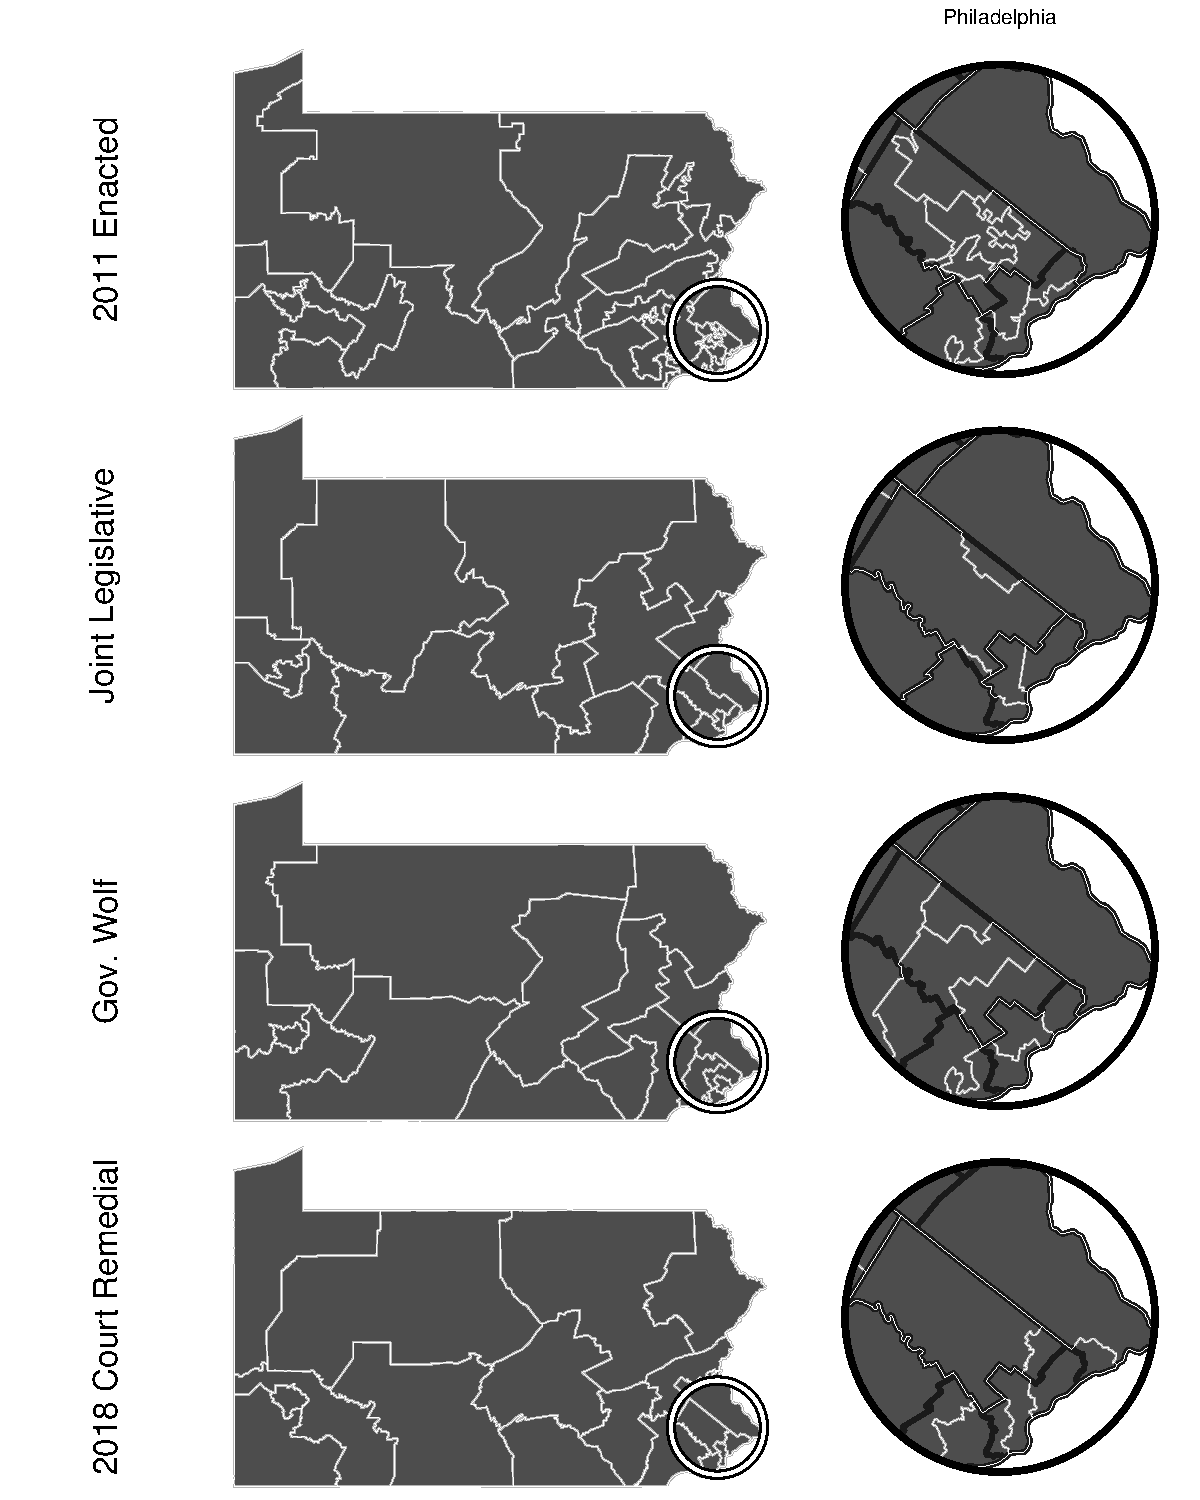
\includegraphics[width=1\textwidth]{Figures/fig_maps.pdf}
    \end{center}
    \tabnotes{Maps a drawn with a Mercator projection. Shapefiles were obtained from the Pennsylvania Supreme Court website for the four government plans.}
\end{figure}
% ---------------------------------------------------------------------
% ▀▄▀▄▀▄ E͎N͎D͎ F͎I͎G͎U͎R͎E͎ ▄▀▄▀▄▀▀▄▀▄▀▄ E͎N͎D͎ F͎I͎G͎U͎R͎E͎ ▄▀▄▀▄▀▀▄▀▄▀▄ E͎N͎D͎ F͎I͎G͎U͎R͎E͎ ▄▀▄
% =====================================================================
        \begin{center} INSERT FIGURE \ref{fig:maps} ABOUT HERE \end{center}
% ---------------------------------------------------------------------
% ▀▄▀▄▀▄ E͎N͎D͎ F͎I͎G͎U͎R͎E͎ ▄▀▄▀▄▀▀▄▀▄▀▄ E͎N͎D͎ F͎I͎G͎U͎R͎E͎ ▄▀▄▀▄▀▀▄▀▄▀▄ E͎N͎D͎ F͎I͎G͎U͎R͎E͎ ▄▀▄
% ===================================================================== 
\par
%
%%%%%%%%%%%%%%%%%%%%%%%%%%%%%%%%%%%%%%%%%%%%%%%%%%%%%%%%%%%%%%%%%%%%
% ↤↤↤↤↤ -------------- S̟U̟B̟-S̟U̟B̟S̟E̟C̟T̟I̟O̟N̟ -------------- ↦↦↦↦↦
            \subsubsection*{Compactness}
% •••••••••••••••••••••••••••••••••••••••••••••••••••••••••••••••••
    The measurement of compactness has long been a central issue in the districting literature \citep[see e.g.,][]{Reock1961, Niemi1990, Polsby1991, Webster2013, Kaufman2018}. Indeed, the original gerrymander was assumed to be evidence of political manipulation because of its irregular shape \citep{Martis2008}. Some minimal level of compactness can make it harder to gerrymander \citep[][cf. \citealt{Webster2013}]{Reock1961, Altman1998}. But compactness is not a magic wand that rules out the possibility of political manipulation. Moreover, as many authors have shown, compactness has multiple dimensions, and these different dimensions need not move in parallel with one another; thus a plan appears compact on one dimension might appear ill-compact on another. The two most common ideas of compactness refer, on the one hand, to how close a legislative district’s boundaries are to its geographic center and, on the other, to how ``regular'' in shape a district appears to be \citep{Niemi1990, Kaufman2018}. In Table \ref{tab:summaries} we report two well-known measures which tap respectively each of these two dimensions. The \textit{Polsby-Popper} measure looks at perimeter irregularity by examining the area of the district compared to that of a circle with similar perimeter, while the \textit{Reock} measure compares the area of a district with that of the district’s circumscribing circle \citep{Reock1961, Polsby1991}. 
% ================================================================= 
% -- FOOTNOTE -- FOOTNOTE -- FOOTNOTE -- FOOTNOTE -- FOOTNOTE --  %
% -----------------------------------------------------------------
        \footnote{$ A_D $ = area of district, $P_D$= perimeter of district, $Circle_D$= minimum circumscribing circle; \\
        \textit{POLSBYPOPPER} = $\frac{4 \pi A_D}{{P_{D}}^{2}}$ \quad
        \textit{REOCK} = $\frac{A_D}{A(Circle_D)}$}
% ----------------------------------------------------------------- 
% -- END FOOTNOTE -- END FOOTNOTE -- END FOOTNOTE -- END FOOTNOTE %
% =================================================================
\par
    The 2011 Enacted map looks awful by both compactness measures compared to the Court-ordered map, or even compared to the two proposed remedial maps; while both the Republican and the Democratic proposed remedial maps look reasonable by both compactness measures, even though the Democratic plan is superior to the Republican plan and the court-ordered map is superior to both. However, until we examine the likely partisan effects of these four plans we are not in a position to conclusively rule out the possibility that one or more of the remedial plans is a ``\textit{stealth gerrymander}''. As is now well recognized, gerrymandering can be found even in plans with compact appearing districts, or in a plan with districts that preserve most county borders.
\par
    Each of the three measures in Table \ref{tab:summaries} indicates a very dramatic deviation from good government standards in the 2011 Enacted map. And, each of three metrics order the plans in good government terms from worst to best in exactly the same way, with the worst plan being the 2011 Enacted map, the next worst being the Republican remedy plan, followed by the the Democratic remedy plan, and the very best being the court-ordered map. Moreover, as we will see later, the same ordering of plans is reflected when we examine the partisan implications of the various maps, with the map ordered into place as a remedy by the Pennsylvania Supreme Court close to perfectly neutral in its expected partisan effects once we recognize the implications of the partisan geography in Pennsylvania in ``naturally'' tilting outcomes slightly in a pro-Republican direction because of differences in the degree of geographic concentration of each party’s supporters (see below). Moreover, we show that the proposed Republican remedy plan can be characterized as a ``disguised'' pro-Republican partisan gerrymander -- what we call a ``stealth gerrymander'' -- which is nearly as pernicious in its expected pro-Republican partisan consequences as the 2011 plan whose effects it claims to ``remedy''.
\par
    To give a more intuitive feel for how egregiously ill-compact the 2011 map is compared to the other alternatives we are considering, Figure \ref{fig:maps} shows all four maps in the same scale, in a gray and white format. What is visually apparent from these maps is how aesthetically ``ugly'' the 2011 map is compared to all of its alternatives. But it also clear that three remedy maps that are similar in having relatively few county cuts nonetheless can look quite different in terms of how each configures districts.
% ================================================================= 
% -- FOOTNOTE -- FOOTNOTE -- FOOTNOTE -- FOOTNOTE -- FOOTNOTE --  %
% -----------------------------------------------------------------
        \footnote{This latter point is reinforced if we examine good government maps prepared by \href{https://www.dailykos.com/stories/2018/2/8/1739648/-Pennsylvania-will-soon-redraw-its-House-map-to-end-GOP-gerrymandering-How-would-you-draw-the-lines}{DailyKos} and by the present authors (available upon request).}
% ----------------------------------------------------------------- 
% -- END FOOTNOTE -- END FOOTNOTE -- END FOOTNOTE -- END FOOTNOTE %
% =================================================================
%
%
% •••••••••••••••••••••••••••••••••••••••••••••••••••••••••••••••••
%     ↤↤↤↤↤ -------------- S̟U̟B̟-S̟U̟B̟S̟E̟C̟T̟I̟O̟N̟ -------------- ↦↦↦↦↦
            \subsection*{Asymmetry Measures}
% •••••••••••••••••••••••••••••••••••••••••••••••••••••••••••••••••
    We emphasize that a partisan gerrymandering claim based on statewide political consequences should also provide evidence that the (a) gerrymandering indicators that are found cannot be explained simply by the geographic distribution of each party’s electoral support (e.g., differential concentration of electoral support can lead to what has been called a ``natural gerrymander''), and (b) that the partisan asymmetry in translating votes into seats is not due to chance alone (e.g., many highly competitive seats won by very narrow margins) but can be expected to be durable. With only 18 districts, sensitivity to chance effects is particularly important. 
\par
    Rebuttal to any claims that the partisan asymmetries observed in the consistent outcomes of the 2011 map can be attributed primarily to differential concentration of party voting strengths, or to chance, is found in the expert witness testimony in the case (see esp. the simulations of potential good government maps done by Professor Chen, discussed in detail in the Pennsylvania Supreme Court opinion in the case, and on which the Court placed great reliance). With respect to the durability of the effects of the 2011 map, this plan yielded unchanged 13R-5D results in all three elections where the map was used. To help explain this over time consistency we note that the 2011 Map has primarily safe seats (13 of 18 won with greater than a 10 percentage point margin). But, indicative of the pro-Republican gerrymander achieved with the 2011 map, those safe seats are distributed in a highly asymmetric fashion, with nine essentially safe seats for Republicans and only four for Democrats.
%        =================================================================
%        -- FOOTNOTE -- FOOTNOTE -- FOOTNOTE -- FOOTNOTE -- FOOTNOTE --  %
% ------------------------------------------------------------------------
        \footnote{However, we should note that some authors \citep[e.g.,][]{Grofman2019_ELJ} have argued that a partisan gerrymandering claim at a jurisdiction-wide level must also be reinforced by district specific evidence of manipulation of particular district boundaries. As noted earlier, we do not discuss this type of district specific evidence here, other than to point out that such evidence was presented at the trial, and that this evidence was used to support the Court’s finding that the Pennsylvania congressional map was an unconstitutional gerrymander under Pennsylvania state law.}
% ------------------------------------------------------------------------
%        -- END FOOTNOTE -- END FOOTNOTE -- END FOOTNOTE -- END FOOTNOTE %
%        =================================================================
%
\par
    There are several metrics that have been proposed to look at the degree to which there is asymmetry in seats-votes relationships that might be indicative of partisan gerrymandering: (1) \textit{partisan bias} \citep{Tufte1973}, (2) the \textit{mean-minus-median} gap \citep{Mcdonald_Best_2015_ELJ} (3) the \textit{efficiency gap} \citep{Stephanopoulos2014_UofChicagoLaw}, and most recently (4) \textit{declination} \citep{Warrington2018}. Each of these measures can be directly calculated for the 2011 map based on district election outcomes in 2012, 2014, and 2016.
% ================================================================= 
% -- FOOTNOTE -- FOOTNOTE -- FOOTNOTE -- FOOTNOTE -- FOOTNOTE --  %
% -----------------------------------------------------------------
        \footnote{Another recently proposed measure is a simplified version of partisan bias which lacks the advantage of separately calculating bias and responsiveness (swing ratio). It is calculated by taking the average two-party vote for the dominant party and adjusting it uniformly downward in each district so that the two parties receive exactly 50\% of the overall vote; then we look to see how far the seat share the dominant party now receives is from 50\% \citep{Wang2016_SLR}.}
% ----------------------------------------------------------------- 
% -- END FOOTNOTE -- END FOOTNOTE -- END FOOTNOTE -- END FOOTNOTE %
% =================================================================
    \underline{Positive} values favor Republicans, while \underline{negative} values favor Democrats. 
\par
    We now define these four measures of gerrymandering with which we will evaluate the four competing maps.
%
% •••••••••••••••••••••••••••••••••••••••••••••••••••••••••••••••••
%     ↤↤↤↤↤ -------------- S̟U̟B̟-S̟U̟B̟S̟E̟C̟T̟I̟O̟N̟ -------------- ↦↦↦↦↦
            \subsubsection*{Partisan Bias}
% •••••••••••••••••••••••••••••••••••••••••••••••••••••••••••••••••
%
    \textit{Partisan Bias} indicates asymmetry in the translation of each party’s votes into seats. Customarily, partisan bias is measured at the (hypothetical) point where each party’s share of the two-party vote is exactly 50\%. At that point, both parties should, by symmetry, receive identical seats shares. Thus, the difference between a party’s projected seat-share with 50\% of the vote and exactly 50\% can be taken as a measure of partisan bias. Note, however, that although a plan must be proportional at the ($50,50$) point, a partisan bias of zero does \underline{not} imply proportional representational. What partisan bias taps is the differential treatment of parties. Thus, for example, if party R gets 61\% of the seats with 52\% of the vote, this is not a sign of bias as long as party L also can be expected to get 61\% of the seats were it to have 52\% of the vote.
% ================================================================= 
% -- FOOTNOTE -- FOOTNOTE -- FOOTNOTE -- FOOTNOTE -- FOOTNOTE --  %
% -----------------------------------------------------------------
        \footnote{Although the basic idea goes back at least as far as \citet{Dahl1956}, the modern \textit{locus classicus} in political science for the idea of partisan bias (and the parallel concept of responsiveness/swing ratio) is \citet{Tufte1973}, with important recent work done by Gary King (see e.g., \citep{GelmanKing1994_unifiedAJPS}; and reviewed in \citet{GrofmanKing2007_ELJ}). A closely related line of research is found in the political geography literature (with \textit{locus classicus} \citet{Brookes1959, Brookes1960} -- with some further methodological improvements by scholars such as \citet{Johnston1994, Rossiter1997}, and \citet{Johnston2002}.}   
% ----------------------------------------------------------------- 
% -- END FOOTNOTE -- END FOOTNOTE -- END FOOTNOTE -- END FOOTNOTE %
% =================================================================
\par
    There are a number of different ways to estimate partisan bias based on the shape of the votes to seats distribution \citep{Tufte1973, Grofman1983, Browning_King_1987_seats_votes, GelmanKing1994_unifiedAJPS, Grofman_et_al_1997_SwingRatio_Bias, Zingher2016_bias_swingratio_JEPP}. The method we use here is that of \citet{Tufte1973}. Hypothetical elections are constructed by incrementally adding (or subtracting) one percentage point (on average) at a time to find aggregate seat outcomes under differing mean vote shares. The resulting ($s$, $v$) points on the votes-to-seats curve are then converted to a log odds form by using $ log(\frac{s}{1-s}) $ as the dependent variable, and $ log(\frac{v}{1-v}) $ as the independent variable. A regression on the transformed variables is then run, with transformed $s$ as the dependent variable, for $v$ values in some range near a 50\% vote share. 
% ================================================================= 
% -- FOOTNOTE -- FOOTNOTE -- FOOTNOTE -- FOOTNOTE -- FOOTNOTE --  %
% -----------------------------------------------------------------    
        \footnote{Where to center the \textit{seats/votes} curve is an unresolved issue in the literature. In \citet{GelmanKing1994_unifiedAJPS} \texttt{JudgeIt} program, the choice is to center the election at the average Democratic vote share over recent elections. \citet{Kastellec_et_al_2008_PS} similarly simulates data for average vote shares between 45\% and 55\%. We checked for consistency between the methods by running the numbers in three ways: centering the simulated outcomes at an average election vote share, centering the simulated outcomes at a tied 50/50 election, and centering the simulated outcomes at the actual election results in the particular election. All three variations provide similar estimates, as do the results from \texttt{JudgeIt}. Readers should note that, with only 18 districts, too much weight should not be placed on the exact bias coefficients reported [see the discussion in \citet{Browning_King_1987_seats_votes}]; but the relative magnitude of the bias values across the different plans is fully congruent with the evaluations of probable partisan gerrymandering yielded by the other measures. Because of the limited number of districts in the plans, the same caution is urged for all the measures of gerrymandering reported in this essay. We have devoted more space to partisan bias than to the other measures of gerrymandering reported in this essay due to it's complexity than to the other more straightforward measures.} 
% ----------------------------------------------------------------- 
% -- END FOOTNOTE -- END FOOTNOTE -- END FOOTNOTE -- END FOOTNOTE %
% =================================================================
    \textit{Partisan Bias} is then calculated from the intercept of this regression using an exponential transformation (for details see \citet{Grofman1983}).
\par
%     ↤↤↤↤↤ -------------- S̟U̟B̟-S̟U̟B̟S̟E̟C̟T̟I̟O̟N̟ -------------- ↦↦↦↦↦
            \subsubsection*{Mean-Median Gap}
% •••••••••••••••••••••••••••••••••••••••••••••••••••••••••••••••••
    When districts are sorted according to two-party vote share, the \textit{Mean-Median Gap} is the difference between the average vote percentage for a party and its vote share in the median district \citep[see][]{Best2018}. This measure is a variant of \textit{skewness}. When the mean is substantially higher or lower than the median, this is taken to be indicative of partisan bias.
\par
%     ↤↤↤↤↤ -------------- S̟U̟B̟-S̟U̟B̟S̟E̟C̟T̟I̟O̟N̟ -------------- ↦↦↦↦↦
            \subsubsection*{Efficiency Gap}
% •••••••••••••••••••••••••••••••••••••••••••••••••••••••••••••••••
    The \textit{Efficiency Gap} is calculated as defined in \citet{Stephanopoulos2014_UofChicagoLaw}, where all the party’s votes are wasted if they lose the district, and all the winner’s votes over 50\% are wasted. The difference between each party’s wasted votes is then divided by the total votes cast to produce the \textit{efficiency gap}, with a value of zero denoting what is regarded as ideal. As noted in \citet[][p. 13]{Best2018}, this is equivalent to taking an aggregate responsiveness (swing ratio) of two as ideal. 
\par
%     ↤↤↤↤↤ -------------- S̟U̟B̟-S̟U̟B̟S̟E̟C̟T̟I̟O̟N̟ -------------- ↦↦↦↦↦
            \subsubsection*{Declination}
% •••••••••••••••••••••••••••••••••••••••••••••••••••••••••••••••••
    Among the more recent measures of gerrymandering is the \textit{Declination}. \textit{Declination} is an astronomical term referring to the angle on a compass, with a Latin root meaning ``a bending away''. For gerrymandering, it uses the angles created from ordering all of the districts by vote share, computing the mean vote-share for each party separately for the seats they won, and then comparing the differences in their distribution. To compare, a line is draw from the mean vote-share to the 0.5 line separately for each party. The angle formed from the different slopes of the line is called the \textit{declination}. An angle indicates whether a plan is a gerrymandering, under the logic that vote-shares should be distributed in some uniform manner across districts. If partisan are \textit{packed}, the angle will be greater. All values range between -1 and 1. Though we have defined the vote-share in terms of Republican outcomes, we adjusted the values such that \underline{negative} values are favorable to the Democrats. Further information on declination can be found in \citet{Warrington2018}.  
\par
\par
    In our view, none of these four measures standing alone can be taken to be proof of gerrymandering. Rather we see them as potentially reinforcing indicators. Our own analyses have found hypotheticals where these measures can generate either a false positive or a false negative, but we have also found that consistent bias in the same direction is unlikely when we use multiple indicators (data omitted for space reasons). We will return to a discussion of the results later in this essay. Here we point out, however, all four indicators point clearly and overwhelmingly in the same direction vis-à-vis the 2011 Enacted plan, as Table \ref{tab:congsum} distinctly shows -- namely that it is a blatant pro-Republican partisan gerrymander.
\par
% •••••••••••••••••••••••••••••••••••••••••••••••••••••••••••••••••••••
% ▀▄▀▄▀▄ SUBSECTION -- SUBSECTION -- SUBSECTION -- SUBSECTION -- ▄▀▄▀▄▀
% •••••••••••••••••••••••••••••••••••••••••••••••••••••••••••••••••••••
    \subsection*{Evaluation of the 2011 enacted map}
% •••••••••••••••••••••••••••••••••••••••••••••••••••••••••••••••••••••
%
%     ↤↤↤↤↤ -------------- S̟U̟B̟-S̟U̟B̟S̟E̟C̟T̟I̟O̟N̟ -------------- ↦↦↦↦↦
        \subsubsection*{Partisan results in actual congressional elections held under the 2011 map}
% •••••••••••••••••••••••••••••••••••••••••••••••••••••••••••••••••
%
    The best evidence about a plan’s partisan consequences is, of course, evidence derived from actual elections under the plan -- if there are any -- though we do need to check if there are highly anomalous aspects to one or more of these elections which would make results from them hard to generalize. Also, the existence of incumbency advantage can have a distorting effect on the translation of votes into seats, since incumbents may deter strong challengers, thus reducing the vote-share of the minority party \citep{Jacobson_Kernell_1981, Abramowitz1991}. Nonetheless, simply from examining outcomes in the three elections held under the plan (2012, 2014, 2016), the claim that the 2011 Pennsylvania congressional plan is an egregious partisan gerrymander is very hard to refute since (a) regardless of voter preferences the plan returned 13 Republicans and 5 Democrats, with no district changing hands over the course of the three elections, and (b) in those three elections, Democrats won only 28\% of the seats (5 out of 18), despite winning a substantial share of the vote in all three elections. In 2012, the Democratic share of the average two-party vote in the congressional elections in Pennsylvania was 48.0\%, in 2014 it was 44.5\%, and in 2016 it was 45.8\%. 
% ================================================================= 
% -- FOOTNOTE -- FOOTNOTE -- FOOTNOTE -- FOOTNOTE -- FOOTNOTE --  %
% -----------------------------------------------------------------
        \footnote{For consistency, we report the average vote share after imputing 0.25 and 0.75 for uncontested districts. In raw votes, Democrats won more votes than Republicans in 2012, and the difference is an artifact of the plan's `packing' and `cracking'. The Democratic raw vote shares are 50.8\% in 2012, 44.5\% in 2014, and 45.9\% in 2016.}
% ----------------------------------------------------------------- 
% -- END FOOTNOTE -- END FOOTNOTE -- END FOOTNOTE -- END FOOTNOTE %
% =================================================================    
    Thus, the discrepancy between Republican vote share and Republican seat share was huge, and yet the seat share appeared to be immutable. Table \ref{tab:congsum} shows the indicators of statewide partisan gerrymandering effects that provides additional compelling evidence of the 2011 map as an (enduring) partisan gerrymander.   
\par
% =====================================================================
% ▀▄▀▄▀▄ T̟A̟B̟L̟E̟ ▄▀▄▀▄▀▀▄▀▄▀▄ T̟A̟B̟L̟E̟ ▄▀▄▀▄▀▀▄▀▄▀▄ T̟A̟B̟L̟E̟ ▄▀▄▀▄▀▀▄▀▄▀▄ T̟A̟B̟L̟E̟
% ---------------------------------------------------------------------
    

% =====================================================================
% ▀▄▀▄▀▄ T̟A̟B̟L̟E̟ ▄▀▄▀▄▀▀▄▀▄▀▄ T̟A̟B̟L̟E̟ ▄▀▄▀▄▀▀▄▀▄▀▄ T̟A̟B̟L̟E̟ ▄▀▄▀▄▀▀▄▀▄▀▄ T̟A̟B̟L̟E̟
% ---------------------------------------------------------------------


% =====================================================================
% ▀▄▀▄▀▄ T̟A̟B̟L̟E̟ ▄▀▄▀▄▀▀▄▀▄▀▄ T̟A̟B̟L̟E̟ ▄▀▄▀▄▀▀▄▀▄▀▄ T̟A̟B̟L̟E̟ ▄▀▄▀▄▀▀▄▀▄▀▄ T̟A̟B̟L̟E̟
% ---------------------------------------------------------------------


% =====================================================================
% ▀▄▀▄▀▄ T̟A̟B̟L̟E̟ ▄▀▄▀▄▀▀▄▀▄▀▄ T̟A̟B̟L̟E̟ ▄▀▄▀▄▀▀▄▀▄▀▄ T̟A̟B̟L̟E̟ ▄▀▄▀▄▀▀▄▀▄▀▄ T̟A̟B̟L̟E̟
% ---------------------------------------------------------------------
\input{Tables/_tab_congsum.tex}
 \begin{center}\textbf{INSERT TABLE \ref{tab:congsum} ABOUT HERE} \end{center}
% •••••••••••••••••••••••••••••••••••••••••••••••••••••••••••••••••


% =====================================================================
% ▀▄▀▄▀▄ T̟A̟B̟L̟E̟ ▄▀▄▀▄▀▀▄▀▄▀▄ T̟A̟B̟L̟E̟ ▄▀▄▀▄▀▀▄▀▄▀▄ T̟A̟B̟L̟E̟ ▄▀▄▀▄▀▀▄▀▄▀▄ T̟A̟B̟L̟E̟
% ---------------------------------------------------------------------
\begin{table}[!htbp] \centering 
  \caption{U.S. House Election Summaries \\ \hspace{2cm}(PA 2012-2016 Enacted Map)} 
  \label{tab:congsum} 
\begin{tabular}{@{\extracolsep{-5pt}} ccccc} 
 & 2012 & 2014 & 2016 & AVE \\ 
\hline \\[-1.8ex] 
Seats &  [13R-5D] &  [13R-5D] &  [13R-5D] & [13R-5D] \\ 
Seat \% & 72.2\% & 72.2\% & 72.2\% & 72.0\% \\ 
Votes & 51.1\% & 55.5\% & 54.2\% & 53.3\% \\ 
Bias & 0.13 & 0.1 & 0.11 & 0.11 \\ 
Efficiency Gap & 0.21 & 0.11 & 0.17 & 0.16 \\ 
Mean/Median & 0.06 & 0.06 & 0.06 & 0.06 \\ 
Declination & 0.46 & 0.36 & 0.39 & 0.4 \\ 
\end{tabular}
\tabnotes{Calculations based on actual congressional elections in Pennsylvania under the map found unconstitutional in 2018. Uncontested races are imputed with 0.25 and 0.75 for the respective winners. Un-adjusted Republican two-party vote totals are 49.2\% for 2012, 55.5\% for 2014, and 54.1\% for 2016. All votes are calculated from the Republican perspective of the two-party vote. We've adjusted all gerrymandering measures such that negative numbers indicate bias in favor of the Democrats.}
\end{table}
% ---------------------------------------------------------------------
% ▀▄▀▄▀▄ E͎N͎D͎ T͎A͎B͎L͎E͎ ▄▀▄▀▄▀▀▄▀▄▀▄ E͎N͎D͎ T͎A͎B͎L͎E͎ ▄▀▄▀▄▀▀▄▀▄▀▄ E͎N͎D͎ T͎A͎B͎L͎E͎ ▄▀▄▀▄▀
% ===================================================================== 
 
 

 \begin{center}\textbf{INSERT TABLE \ref{tab:congsum} ABOUT HERE} \end{center}
% •••••••••••••••••••••••••••••••••••••••••••••••••••••••••••••••••


% =====================================================================
% ▀▄▀▄▀▄ T̟A̟B̟L̟E̟ ▄▀▄▀▄▀▀▄▀▄▀▄ T̟A̟B̟L̟E̟ ▄▀▄▀▄▀▀▄▀▄▀▄ T̟A̟B̟L̟E̟ ▄▀▄▀▄▀▀▄▀▄▀▄ T̟A̟B̟L̟E̟
% ---------------------------------------------------------------------
\begin{table}[!htbp] \centering 
  \caption{U.S. House Election Summaries \\ \hspace{2cm}(PA 2012-2016 Enacted Map)} 
  \label{tab:congsum} 
\begin{tabular}{@{\extracolsep{-5pt}} ccccc} 
 & 2012 & 2014 & 2016 & AVE \\ 
\hline \\[-1.8ex] 
Seats &  [13R-5D] &  [13R-5D] &  [13R-5D] & [13R-5D] \\ 
Seat \% & 72.2\% & 72.2\% & 72.2\% & 72.0\% \\ 
Votes & 51.1\% & 55.5\% & 54.2\% & 53.3\% \\ 
Bias & 0.13 & 0.1 & 0.11 & 0.11 \\ 
Efficiency Gap & 0.21 & 0.11 & 0.17 & 0.16 \\ 
Mean/Median & 0.06 & 0.06 & 0.06 & 0.06 \\ 
Declination & 0.46 & 0.36 & 0.39 & 0.4 \\ 
\end{tabular}
\tabnotes{Calculations based on actual congressional elections in Pennsylvania under the map found unconstitutional in 2018. Uncontested races are imputed with 0.25 and 0.75 for the respective winners. Un-adjusted Republican two-party vote totals are 49.2\% for 2012, 55.5\% for 2014, and 54.1\% for 2016. All votes are calculated from the Republican perspective of the two-party vote. We've adjusted all gerrymandering measures such that negative numbers indicate bias in favor of the Democrats.}
\end{table}
% ---------------------------------------------------------------------
% ▀▄▀▄▀▄ E͎N͎D͎ T͎A͎B͎L͎E͎ ▄▀▄▀▄▀▀▄▀▄▀▄ E͎N͎D͎ T͎A͎B͎L͎E͎ ▄▀▄▀▄▀▀▄▀▄▀▄ E͎N͎D͎ T͎A͎B͎L͎E͎ ▄▀▄▀▄▀
% ===================================================================== 
 
 

 \begin{center}\textbf{INSERT TABLE \ref{tab:congsum} ABOUT HERE} \end{center}
% •••••••••••••••••••••••••••••••••••••••••••••••••••••••••••••••••


% =====================================================================
% ▀▄▀▄▀▄ T̟A̟B̟L̟E̟ ▄▀▄▀▄▀▀▄▀▄▀▄ T̟A̟B̟L̟E̟ ▄▀▄▀▄▀▀▄▀▄▀▄ T̟A̟B̟L̟E̟ ▄▀▄▀▄▀▀▄▀▄▀▄ T̟A̟B̟L̟E̟
% ---------------------------------------------------------------------
\begin{table}[!htbp] \centering 
  \caption{U.S. House Election Summaries \\ \hspace{2cm}(PA 2012-2016 Enacted Map)} 
  \label{tab:congsum} 
\begin{tabular}{@{\extracolsep{-5pt}} ccccc} 
 & 2012 & 2014 & 2016 & AVE \\ 
\hline \\[-1.8ex] 
Seats &  [13R-5D] &  [13R-5D] &  [13R-5D] & [13R-5D] \\ 
Seat \% & 72.2\% & 72.2\% & 72.2\% & 72.0\% \\ 
Votes & 51.1\% & 55.5\% & 54.2\% & 53.3\% \\ 
Bias & 0.13 & 0.1 & 0.11 & 0.11 \\ 
Efficiency Gap & 0.21 & 0.11 & 0.17 & 0.16 \\ 
Mean/Median & 0.06 & 0.06 & 0.06 & 0.06 \\ 
Declination & 0.46 & 0.36 & 0.39 & 0.4 \\ 
\end{tabular}
\tabnotes{Calculations based on actual congressional elections in Pennsylvania under the map found unconstitutional in 2018. Uncontested races are imputed with 0.25 and 0.75 for the respective winners. Un-adjusted Republican two-party vote totals are 49.2\% for 2012, 55.5\% for 2014, and 54.1\% for 2016. All votes are calculated from the Republican perspective of the two-party vote. We've adjusted all gerrymandering measures such that negative numbers indicate bias in favor of the Democrats.}
\end{table}
% ---------------------------------------------------------------------
% ▀▄▀▄▀▄ E͎N͎D͎ T͎A͎B͎L͎E͎ ▄▀▄▀▄▀▀▄▀▄▀▄ E͎N͎D͎ T͎A͎B͎L͎E͎ ▄▀▄▀▄▀▀▄▀▄▀▄ E͎N͎D͎ T͎A͎B͎L͎E͎ ▄▀▄▀▄▀
% ===================================================================== 
 
 

        \begin{center}\textbf{INSERT TABLE \ref{tab:congsum} ABOUT HERE} \end{center}
% •••••••••••••••••••••••••••••••••••••••••••••••••••••••••••••••••
%
\par
% •••••••••••••••••••••••••••••••••••••••••••••••••••••••••••••••••••••
% ▀▄▀▄▀▄ SUBSECTION -- SUBSECTION -- SUBSECTION -- SUBSECTION -- ▄▀▄▀▄▀
% •••••••••••••••••••••••••••••••••••••••••••••••••••••••••••••••••••••
    \subsection*{Evaluating district plans using Statewide elections to provide a normal vote baseline}
% •••••••••••••••••••••••••••••••••••••••••••••••••••••••••••••••••••••
%
    In order to assess expected partisan consequences for plans that have not yet been implemented we need to develop a predictive equation, and one such way is with data on partisan outcomes for state-wide elections projected into the new districts. For example, Professor Jowei Chen in his testimony in the Pennsylvania case used a composite of the six state-wide elections between 2008 and 2010 to estimate the political consequences of alternative maps. After extensive investigation of alternative prediction models and their accuracy in reproducing the partisan outcomes of the 2012, 2014, and 2016 congressional elections at the district level (data omitted for space reasons), we have opted for a model that takes the average of five state-wide 2016 elections that reflect a balance of Republican and Democratic success: President, U.S. Senate, PA Attorney General, PA Treasurer, and PA Auditor.
%        =================================================================
%        -- FOOTNOTE -- FOOTNOTE -- FOOTNOTE -- FOOTNOTE -- FOOTNOTE --  %
% ------------------------------------------------------------------------
        \footnote{We use the five-election composite to calculate all four plans. We aggregate voting district level (precincts) data for these five statewide elections and project them to the three maps in which we are comparing the 2011 enacted map.}
% ------------------------------------------------------------------------
%        -- END FOOTNOTE -- END FOOTNOTE -- END FOOTNOTE -- END FOOTNOTE %
%        =================================================================
%    
    Republicans won the statewide vote in two of them (President, U.S. Senate), while the Democrats won the statewide vote in three of them (Auditor, Treasurer, and Attorney General). The average vote for the Republicans across these five elections was 49.1\%.
%        ================================================================= 
%        -- FOOTNOTE -- FOOTNOTE -- FOOTNOTE -- FOOTNOTE -- FOOTNOTE --  %
% ------------------------------------------------------------------------
    \footnote{We report the Republican share of the two-party vote ($\delta_{i}$). Districting plans are represented by $\mathcal D $, (e.g., $\mathcal D_{enacted}$, $\mathcal D_{remedial}$, \dots, $\mathcal D_{j}$), and each election in year $ y $ has a district vote distribution $ \Delta_{y} = [\delta_{y1}, \delta_{y2}, \dots, \delta_{yi}] $. To find the overall state-wide vote share, we calculate the average district vote share, $ \bar{\Delta}_{\mathcal D y} = \frac{1}{n}\sum\limits_{i=1}^{n} \delta_{yi} $. By averaging, we reduce the influence of turnout variation among districts. This district-specific average is a useful state-wide estimate of voter sentiment though it is in part effected by the particular configuration of districts being examined \citep[see e.g.][cf. \cite{Grofman_et_al_1997__IntedgratedPerspective_ES}]{Kastellec_et_al_2008_PS}. In particular, incumbency advantage effects affect our ability to accurately predict vote outcomes. In ancillary work not reported here, we have looked at changes in congressional incumbency advantage in Pennsylvania over multiple decades \citep[cf.][]{Jacobson2015}. We compiled the composite measure using both the sum of the raw votes by party and an average of the two-party vote in the five races at the district level (see discussion on alternative ways to tabulate vote-shares in \citet{Grofman_et_al_1997__IntedgratedPerspective_ES}. Both ways result in the same district partisanship outcomes in all plans.}
% ----------------------------------------------------------------- 
% -- END FOOTNOTE -- END FOOTNOTE -- END FOOTNOTE -- END FOOTNOTE %
% =================================================================
\par
    We need to check that our five-election composite offers a plausible basis for a prediction model that accounts for the idiosyncrasies inherent to congressional districts. Encouragingly, our five-election composite results is the same 13R-5D result that the 2016 congressional races delivered. Additionally, each district’s outcome is identical to the 2016 congressional district results when we uniformly adjust in each district the projected vote based on the composite state-wide elections (the ``normal'' vote, without  congressional incumbency effects) by an amount equaling the difference between the statewide legislative vote and the the statewide congressional vote.
\par
    When we look at the five election composite for the 2018 court remedial plan, we need to (a) adjust it for the actual statewide congressional Democratic vote share in 2018, and (b) to take into account this differential incumbency advantage that still benefits Republicans. Without doing so, the outcomes of the Court-ordered plan might have a wide range, with anywhere from a 5R to an 11R outcome possible because of the high number of competitive seats. However, when we take both factors into account by uniformly shifting the state-wide composite to reflect the 2018 statewide two-party congressional vote, and by adding in congressional incumbency advantage, which we have estimated in the 2012-2016 period to be on the order of magnitude of 4.3\% (analyses omitted for space reasons, \citet[see ][]{GelmenKing1990_inc_AJPS}), we get a 9R-9D outcome as the most likely outcome in 2018 under the court-ordered map in our predictive model. Thus, our confidence in the five election projection method is further buttressed when we applied this method to predict the results of the 2018 election under the court-ordered remedial map in the light of the actual statewide aggregate results in 2018, and taking incumbency effects into account. In the congressional elections of 2018, the raw Republican two-party vote share in 2018 was 44.8\%, which represented a Democratic advantage, but not enough to overcome the twin barriers to a Democratic majority of over-concentration of Democratic support in urban areas and continued Republican incumbency advantage.
% ================================================================= 
% -- FOOTNOTE -- FOOTNOTE -- FOOTNOTE -- FOOTNOTE -- FOOTNOTE --- %
% -----------------------------------------------------------------     
        \footnote{Six Republicans and five Democrats ran for re-election after the new map was put in place. No incumbent lost. There were two Republican incumbents who won by less than 2 percentage points, along with one who won by less than 3 percentage points. There was just one seat won by Democrats in 2018 with a margin of 5 percentage points or less. Republicans therefore had four incumbents running and winning in competitive districts compared to just two for Democrats (10+ percentage point margin).}
% ----------------------------------------------------------------- 
% -- END FOOTNOTE -- END FOOTNOTE -- END FOOTNOTE -- END FOOTNOTE %
% =================================================================
    We are not claiming to predict vote shares in advance of an election. We also recognize that the composite of state-wide elections is intended to provide a ``normal vote'' baseline that must be ``corrected'' with incumbency effects if we do wish to actually predict outcomes.
\par
    We must distinguish our ability to assess asymmetry in expected seats-vote relationships based on the ``normal vote'' distribution of party support across districts -- and thus to assess the degree to which a plan is a gerrymander -- from our ability to predict actual election outcomes. The more competitive districts there are in a map, the more results depend strongly on electoral tides, and the greater the potential for winning vote margins in some districts to be small and determined by factors idiosyncratic to a district and by incumbency advantage. The 2011 map has 13 non-competitive districts (10+ percentage point margin) with a clear 9-4 Republican advantage, thus virtually guaranteeing continued Republican dominance regardless of aggregate two party vote share. The Court drawn map, comparatively, had only 8 non-competitive districts, with a balance of 3-R and 5-D. Which party will control the delegation under a highly competitive plan such as the Court-ordered plan depends almost entirely on the state-wide vote share and on incumbency advantage, along with idiosyncratic features of the competitive districts that might be small in magnitude but still matter in highly competitive seats. 
\par
    We wish to do a further robustness check on the plausibility of using our five-election composite to calculate the various metrics designed to measure potential gerrymandering. One way to do this is to see how well the composite (calculated at a hypothetical 50\% vote share) mimics the results of the values for the four metrics for the 2011 map that we previously obtained using the actual congressional election results for that map. What we are doing is comparing a hypothetical ``normal vote'' \citep{Converse1966} assumption (based on a statewide vote in which we are not taking incumbency effects into account) with the average of what we actually get in three different congressional elections. The congressional results for 2012-2016 and an average of the three, reported in Table \ref{tab:congsum}, are 0.11 for partisan bias, 0.16 for the efficiency gap, 0.06 for the value of the mean minus median gap, and 0.40 for \textit{declination}. The comparable results from Table \ref{tab:gerry} for the 2011 enacted map at 50\% vote-share are 0.09, 0.24, 0.05, and 0.39.
%        =================================================================
%        -- FOOTNOTE -- FOOTNOTE -- FOOTNOTE -- FOOTNOTE -- FOOTNOTE --  %
% ------------------------------------------------------------------------
        \footnote{If we center the simulations at the 2016 statewide Republican vote of 53.3\% of the vote, we again get remarkably consistent estimates [0.09, 0.19, 0.05, 0.46].}
% ------------------------------------------------------------------------
%        -- END FOOTNOTE -- END FOOTNOTE -- END FOOTNOTE -- END FOOTNOTE %
%        =================================================================
%
% =================================================================
% -- TABLE -- TABLE -- TABLE -- TABLE -- TABLE -- TABLE -- TABLE  % 
% -----------------------------------------------------------------
    

% =====================================================================
% ▀▄▀▄▀▄ T̟A̟B̟L̟E̟ ▄▀▄▀▄▀▀▄▀▄▀▄ T̟A̟B̟L̟E̟ ▄▀▄▀▄▀▀▄▀▄▀▄ T̟A̟B̟L̟E̟ ▄▀▄▀▄▀▀▄▀▄▀▄ T̟A̟B̟L̟E̟
% ---------------------------------------------------------------------


% =====================================================================
% ▀▄▀▄▀▄ T̟A̟B̟L̟E̟ ▄▀▄▀▄▀▀▄▀▄▀▄ T̟A̟B̟L̟E̟ ▄▀▄▀▄▀▀▄▀▄▀▄ T̟A̟B̟L̟E̟ ▄▀▄▀▄▀▀▄▀▄▀▄ T̟A̟B̟L̟E̟
% ---------------------------------------------------------------------


% =====================================================================
% ▀▄▀▄▀▄ T̟A̟B̟L̟E̟ ▄▀▄▀▄▀▀▄▀▄▀▄ T̟A̟B̟L̟E̟ ▄▀▄▀▄▀▀▄▀▄▀▄ T̟A̟B̟L̟E̟ ▄▀▄▀▄▀▀▄▀▄▀▄ T̟A̟B̟L̟E̟
% ---------------------------------------------------------------------
\input{Tables/_tab_gerry.tex}
 \begin{center}\textbf{INSERT TABLE \ref{tab:gerry} ABOUT HERE} \end{center}
% •••••••••••••••••••••••••••••••••••••••••••••••••••••••••••••••••


% =====================================================================
% ▀▄▀▄▀▄ T̟A̟B̟L̟E̟ ▄▀▄▀▄▀▀▄▀▄▀▄ T̟A̟B̟L̟E̟ ▄▀▄▀▄▀▀▄▀▄▀▄ T̟A̟B̟L̟E̟ ▄▀▄▀▄▀▀▄▀▄▀▄ T̟A̟B̟L̟E̟
% ---------------------------------------------------------------------
\begin{table}[!htbp] \centering 
  \caption{Measures of Gerrymandering for the Four Considered Plans} 
  \label{tab:gerry} 
\begin{tabular}{@{\extracolsep{-5pt}} ccccc} 
 & 2011 Enacted & Joint Legislative & Gov. Wolf & 2018 Court Remedial \\ 
\hline \\[-1.8ex] 
Partisan Bias & 0.09$^{***}$ & 0.08$^{***}$ & 0.06$^{**}$ & 0.04$^{}$ \\ 
 & \textit{[0.05, 0.13]} & \textit{[0.03, 0.12]} & \textit{[0.02, 0.11]} & \textit{[-0.01, 0.08]} \\ 
Efficiency Gap & 0.24$^{***}$ & 0.22$^{**}$ & 0.14$^{}$ & 0.08$^{}$ \\ 
 & \textit{[0.09, 0.36]} & \textit{[0.07, 0.36]} & \textit{[0, 0.3]} & \textit{[-0.07, 0.21]} \\ 
Mean/Median & 0.05$^{***}$ & 0.04$^{**}$ & 0.04$^{*}$ & 0.02$^{}$ \\ 
 & \textit{[0.02, 0.07]} & \textit{[0.01, 0.07]} & \textit{[0, 0.07]} & \textit{[-0.01, 0.05]} \\ 
Declination & 0.39$^{**}$ & 0.33$^{*}$ & 0.21$^{}$ & 0.14$^{}$ \\ 
 & \textit{[0.13, 0.63]} & \textit{[0.07, 0.61]} & \textit{[-0.02, 0.47]} & \textit{[-0.1, 0.42]} \\ 
\end{tabular}
\tabnotes{$^{*}$p $<$ 0.05; $^{**}$p $<$ .01; $^{***}$p $<$ 0.001. Measures are averages of 1,000 simulations for each map using the 2016 composite. Brackets numbers are the 95\% range.}
\end{table}
% ---------------------------------------------------------------------
% ▀▄▀▄▀▄ E͎N͎D͎ T͎A͎B͎L͎E͎ ▄▀▄▀▄▀▀▄▀▄▀▄ E͎N͎D͎ T͎A͎B͎L͎E͎ ▄▀▄▀▄▀▀▄▀▄▀▄ E͎N͎D͎ T͎A͎B͎L͎E͎ ▄▀▄▀▄▀
% ===================================================================== 
 
 

 \begin{center}\textbf{INSERT TABLE \ref{tab:gerry} ABOUT HERE} \end{center}
% •••••••••••••••••••••••••••••••••••••••••••••••••••••••••••••••••


% =====================================================================
% ▀▄▀▄▀▄ T̟A̟B̟L̟E̟ ▄▀▄▀▄▀▀▄▀▄▀▄ T̟A̟B̟L̟E̟ ▄▀▄▀▄▀▀▄▀▄▀▄ T̟A̟B̟L̟E̟ ▄▀▄▀▄▀▀▄▀▄▀▄ T̟A̟B̟L̟E̟
% ---------------------------------------------------------------------
\begin{table}[!htbp] \centering 
  \caption{Measures of Gerrymandering for the Four Considered Plans} 
  \label{tab:gerry} 
\begin{tabular}{@{\extracolsep{-5pt}} ccccc} 
 & 2011 Enacted & Joint Legislative & Gov. Wolf & 2018 Court Remedial \\ 
\hline \\[-1.8ex] 
Partisan Bias & 0.09$^{***}$ & 0.08$^{***}$ & 0.06$^{**}$ & 0.04$^{}$ \\ 
 & \textit{[0.05, 0.13]} & \textit{[0.03, 0.12]} & \textit{[0.02, 0.11]} & \textit{[-0.01, 0.08]} \\ 
Efficiency Gap & 0.24$^{***}$ & 0.22$^{**}$ & 0.14$^{}$ & 0.08$^{}$ \\ 
 & \textit{[0.09, 0.36]} & \textit{[0.07, 0.36]} & \textit{[0, 0.3]} & \textit{[-0.07, 0.21]} \\ 
Mean/Median & 0.05$^{***}$ & 0.04$^{**}$ & 0.04$^{*}$ & 0.02$^{}$ \\ 
 & \textit{[0.02, 0.07]} & \textit{[0.01, 0.07]} & \textit{[0, 0.07]} & \textit{[-0.01, 0.05]} \\ 
Declination & 0.39$^{**}$ & 0.33$^{*}$ & 0.21$^{}$ & 0.14$^{}$ \\ 
 & \textit{[0.13, 0.63]} & \textit{[0.07, 0.61]} & \textit{[-0.02, 0.47]} & \textit{[-0.1, 0.42]} \\ 
\end{tabular}
\tabnotes{$^{*}$p $<$ 0.05; $^{**}$p $<$ .01; $^{***}$p $<$ 0.001. Measures are averages of 1,000 simulations for each map using the 2016 composite. Brackets numbers are the 95\% range.}
\end{table}
% ---------------------------------------------------------------------
% ▀▄▀▄▀▄ E͎N͎D͎ T͎A͎B͎L͎E͎ ▄▀▄▀▄▀▀▄▀▄▀▄ E͎N͎D͎ T͎A͎B͎L͎E͎ ▄▀▄▀▄▀▀▄▀▄▀▄ E͎N͎D͎ T͎A͎B͎L͎E͎ ▄▀▄▀▄▀
% ===================================================================== 
 
 

 \begin{center}\textbf{INSERT TABLE \ref{tab:gerry} ABOUT HERE} \end{center}
% •••••••••••••••••••••••••••••••••••••••••••••••••••••••••••••••••


% =====================================================================
% ▀▄▀▄▀▄ T̟A̟B̟L̟E̟ ▄▀▄▀▄▀▀▄▀▄▀▄ T̟A̟B̟L̟E̟ ▄▀▄▀▄▀▀▄▀▄▀▄ T̟A̟B̟L̟E̟ ▄▀▄▀▄▀▀▄▀▄▀▄ T̟A̟B̟L̟E̟
% ---------------------------------------------------------------------
\begin{table}[!htbp] \centering 
  \caption{Measures of Gerrymandering for the Four Considered Plans} 
  \label{tab:gerry} 
\begin{tabular}{@{\extracolsep{-5pt}} ccccc} 
 & 2011 Enacted & Joint Legislative & Gov. Wolf & 2018 Court Remedial \\ 
\hline \\[-1.8ex] 
Partisan Bias & 0.09$^{***}$ & 0.08$^{***}$ & 0.06$^{**}$ & 0.04$^{}$ \\ 
 & \textit{[0.05, 0.13]} & \textit{[0.03, 0.12]} & \textit{[0.02, 0.11]} & \textit{[-0.01, 0.08]} \\ 
Efficiency Gap & 0.24$^{***}$ & 0.22$^{**}$ & 0.14$^{}$ & 0.08$^{}$ \\ 
 & \textit{[0.09, 0.36]} & \textit{[0.07, 0.36]} & \textit{[0, 0.3]} & \textit{[-0.07, 0.21]} \\ 
Mean/Median & 0.05$^{***}$ & 0.04$^{**}$ & 0.04$^{*}$ & 0.02$^{}$ \\ 
 & \textit{[0.02, 0.07]} & \textit{[0.01, 0.07]} & \textit{[0, 0.07]} & \textit{[-0.01, 0.05]} \\ 
Declination & 0.39$^{**}$ & 0.33$^{*}$ & 0.21$^{}$ & 0.14$^{}$ \\ 
 & \textit{[0.13, 0.63]} & \textit{[0.07, 0.61]} & \textit{[-0.02, 0.47]} & \textit{[-0.1, 0.42]} \\ 
\end{tabular}
\tabnotes{$^{*}$p $<$ 0.05; $^{**}$p $<$ .01; $^{***}$p $<$ 0.001. Measures are averages of 1,000 simulations for each map using the 2016 composite. Brackets numbers are the 95\% range.}
\end{table}
% ---------------------------------------------------------------------
% ▀▄▀▄▀▄ E͎N͎D͎ T͎A͎B͎L͎E͎ ▄▀▄▀▄▀▀▄▀▄▀▄ E͎N͎D͎ T͎A͎B͎L͎E͎ ▄▀▄▀▄▀▀▄▀▄▀▄ E͎N͎D͎ T͎A͎B͎L͎E͎ ▄▀▄▀▄▀
% ===================================================================== 
 
 

        \begin{center}\textbf{INSERT TABLE \ref{tab:gerry} ABOUT HERE} \end{center}
% •••••••••••••••••••••••••••••••••••••••••••••••••••••••••••••••••
\par
    The findings from Table \ref{tab:gerry} are very clear; regardless of which metric we examine, the 2011 map is the most gerrymandered. Not surprisingly, the nature of the bias is in a pro-Republican direction. Given the cumulative weight of all the evidence, the 2011 congressional map was clearly an egregious pro-Republican gerrymander. All four measures of potential gerrymandering are statistically significant for the 2011 map using the composite simulations. In contrast, as we might expect, the court-ordered plan, prepared by a respected expert whose instructions were to satisfy good government criteria, was by a considerable margin the closest to a perfectly neutral plan in partisan terms according to all four measures. Indeed, none of the four measures of potential gerrymandering is statistically significant for the court-ordered map. And when we turn to the Republican Joint Legislative plan we find that all four measures are again statistically significant.  
\par
    Finally, we return to the plan offered by the Democratic governor, Governor Wolf. To our surprise, this plan appeared to have a pro-Republican tilt, though not to the same extent as either the 2011 enacted plan or the Republican alternative. This somewhat puzzling finding suggests that the Governor might have been under pressure from Democratic incumbents not to reduce their expected vote margins, or that he sincerely intended it to be a compromise that the Republican legislature might agree to. However, as shown in \ref{tab:gerry}, two of the apparent pro-Republican indicators for the plan are statistically insignificant. Moreover, there is one important difference between the joint plan and that of the Governor: among the seven districts likely to be won by Democrats, the Democratic percentages are cut more narrowly in the Republican plan than in the Governor’s plan in three of the districts so that, in a good Republican year, Republicans will do better under their plan than under the Democratic plan.
\par
% =================================================================
% -- TABLE -- TABLE -- TABLE -- TABLE -- TABLE -- TABLE -- TABLE  % 
% -----------------------------------------------------------------
    

% =====================================================================
% ▀▄▀▄▀▄ T̟A̟B̟L̟E̟ ▄▀▄▀▄▀▀▄▀▄▀▄ T̟A̟B̟L̟E̟ ▄▀▄▀▄▀▀▄▀▄▀▄ T̟A̟B̟L̟E̟ ▄▀▄▀▄▀▀▄▀▄▀▄ T̟A̟B̟L̟E̟
% ---------------------------------------------------------------------


% =====================================================================
% ▀▄▀▄▀▄ T̟A̟B̟L̟E̟ ▄▀▄▀▄▀▀▄▀▄▀▄ T̟A̟B̟L̟E̟ ▄▀▄▀▄▀▀▄▀▄▀▄ T̟A̟B̟L̟E̟ ▄▀▄▀▄▀▀▄▀▄▀▄ T̟A̟B̟L̟E̟
% ---------------------------------------------------------------------


% =====================================================================
% ▀▄▀▄▀▄ T̟A̟B̟L̟E̟ ▄▀▄▀▄▀▀▄▀▄▀▄ T̟A̟B̟L̟E̟ ▄▀▄▀▄▀▀▄▀▄▀▄ T̟A̟B̟L̟E̟ ▄▀▄▀▄▀▀▄▀▄▀▄ T̟A̟B̟L̟E̟
% ---------------------------------------------------------------------
\input{Tables/_tab_prob.tex}
 \begin{center}\textbf{INSERT TABLE \ref{tab:prob} ABOUT HERE} \end{center}
% •••••••••••••••••••••••••••••••••••••••••••••••••••••••••••••••••


% =====================================================================
% ▀▄▀▄▀▄ T̟A̟B̟L̟E̟ ▄▀▄▀▄▀▀▄▀▄▀▄ T̟A̟B̟L̟E̟ ▄▀▄▀▄▀▀▄▀▄▀▄ T̟A̟B̟L̟E̟ ▄▀▄▀▄▀▀▄▀▄▀▄ T̟A̟B̟L̟E̟
% ---------------------------------------------------------------------
\begin{landscape}
\begin{table}[!htbp] \centering 
  \caption{Probabilistic Projections of Partisan Outcomes for Four Plans at 50\% Vote-Share} 
  \label{tab:prob} 
\begin{tabular}{@{\extracolsep{-5pt}} ccccc} 
 & 2011 Enacted & Joint Legislative & Gov. Wolf & 2018 Court Remedial \\ 
\hline \\[-1.8ex] 
Mean Seat Share & 12.23R-5.77D & 11.69R-6.31D & 10.81R-7.19D & 10.2R-7.8D \\ 
SDS & (10.8R-7.2D, 14.4R-3.6D) & (9R-9D, 14.4R-3.6D) & (9R-9D, 12.6R-5.4D) & (7.2R-10.8D, 12.6R-5.4D) \\ 
Median Seat Share & 12R-6D & 12R-6D & 11R-7D & 10R-8D \\ 
Probability Republican Majority & 98.6\% & 97.3\% & 88.3\% & 69.4\% \\ 
Probability Democratic Majority & 0.3\% & 0.3\% & 2.0\% & 6.6\% \\ 
Probability Tied Delegation & 1.1\% & 2.4\% & 9.7\% & 24.0\% \\ 
\end{tabular}
\tabnotes{Using a Composite of Five Statewide Elections (adjusted to a 50\% Vote Share) but not correcting for incumbency. We report the mean seat-share from 1,000 simulations, along with a 95\% range of the simulated outcomes.}
\end{table}
\end{landscape}
% ---------------------------------------------------------------------
% ▀▄▀▄▀▄ E͎N͎D͎ T͎A͎B͎L͎E͎ ▄▀▄▀▄▀▀▄▀▄▀▄ E͎N͎D͎ T͎A͎B͎L͎E͎ ▄▀▄▀▄▀▀▄▀▄▀▄ E͎N͎D͎ T͎A͎B͎L͎E͎ ▄▀▄▀▄▀
% ===================================================================== 
 
 

 \begin{center}\textbf{INSERT TABLE \ref{tab:prob} ABOUT HERE} \end{center}
% •••••••••••••••••••••••••••••••••••••••••••••••••••••••••••••••••


% =====================================================================
% ▀▄▀▄▀▄ T̟A̟B̟L̟E̟ ▄▀▄▀▄▀▀▄▀▄▀▄ T̟A̟B̟L̟E̟ ▄▀▄▀▄▀▀▄▀▄▀▄ T̟A̟B̟L̟E̟ ▄▀▄▀▄▀▀▄▀▄▀▄ T̟A̟B̟L̟E̟
% ---------------------------------------------------------------------
\begin{landscape}
\begin{table}[!htbp] \centering 
  \caption{Probabilistic Projections of Partisan Outcomes for Four Plans at 50\% Vote-Share} 
  \label{tab:prob} 
\begin{tabular}{@{\extracolsep{-5pt}} ccccc} 
 & 2011 Enacted & Joint Legislative & Gov. Wolf & 2018 Court Remedial \\ 
\hline \\[-1.8ex] 
Mean Seat Share & 12.23R-5.77D & 11.69R-6.31D & 10.81R-7.19D & 10.2R-7.8D \\ 
SDS & (10.8R-7.2D, 14.4R-3.6D) & (9R-9D, 14.4R-3.6D) & (9R-9D, 12.6R-5.4D) & (7.2R-10.8D, 12.6R-5.4D) \\ 
Median Seat Share & 12R-6D & 12R-6D & 11R-7D & 10R-8D \\ 
Probability Republican Majority & 98.6\% & 97.3\% & 88.3\% & 69.4\% \\ 
Probability Democratic Majority & 0.3\% & 0.3\% & 2.0\% & 6.6\% \\ 
Probability Tied Delegation & 1.1\% & 2.4\% & 9.7\% & 24.0\% \\ 
\end{tabular}
\tabnotes{Using a Composite of Five Statewide Elections (adjusted to a 50\% Vote Share) but not correcting for incumbency. We report the mean seat-share from 1,000 simulations, along with a 95\% range of the simulated outcomes.}
\end{table}
\end{landscape}
% ---------------------------------------------------------------------
% ▀▄▀▄▀▄ E͎N͎D͎ T͎A͎B͎L͎E͎ ▄▀▄▀▄▀▀▄▀▄▀▄ E͎N͎D͎ T͎A͎B͎L͎E͎ ▄▀▄▀▄▀▀▄▀▄▀▄ E͎N͎D͎ T͎A͎B͎L͎E͎ ▄▀▄▀▄▀
% ===================================================================== 
 
 

 \begin{center}\textbf{INSERT TABLE \ref{tab:prob} ABOUT HERE} \end{center}
% •••••••••••••••••••••••••••••••••••••••••••••••••••••••••••••••••


% =====================================================================
% ▀▄▀▄▀▄ T̟A̟B̟L̟E̟ ▄▀▄▀▄▀▀▄▀▄▀▄ T̟A̟B̟L̟E̟ ▄▀▄▀▄▀▀▄▀▄▀▄ T̟A̟B̟L̟E̟ ▄▀▄▀▄▀▀▄▀▄▀▄ T̟A̟B̟L̟E̟
% ---------------------------------------------------------------------
\begin{landscape}
\begin{table}[!htbp] \centering 
  \caption{Probabilistic Projections of Partisan Outcomes for Four Plans at 50\% Vote-Share} 
  \label{tab:prob} 
\begin{tabular}{@{\extracolsep{-5pt}} ccccc} 
 & 2011 Enacted & Joint Legislative & Gov. Wolf & 2018 Court Remedial \\ 
\hline \\[-1.8ex] 
Mean Seat Share & 12.23R-5.77D & 11.69R-6.31D & 10.81R-7.19D & 10.2R-7.8D \\ 
SDS & (10.8R-7.2D, 14.4R-3.6D) & (9R-9D, 14.4R-3.6D) & (9R-9D, 12.6R-5.4D) & (7.2R-10.8D, 12.6R-5.4D) \\ 
Median Seat Share & 12R-6D & 12R-6D & 11R-7D & 10R-8D \\ 
Probability Republican Majority & 98.6\% & 97.3\% & 88.3\% & 69.4\% \\ 
Probability Democratic Majority & 0.3\% & 0.3\% & 2.0\% & 6.6\% \\ 
Probability Tied Delegation & 1.1\% & 2.4\% & 9.7\% & 24.0\% \\ 
\end{tabular}
\tabnotes{Using a Composite of Five Statewide Elections (adjusted to a 50\% Vote Share) but not correcting for incumbency. We report the mean seat-share from 1,000 simulations, along with a 95\% range of the simulated outcomes.}
\end{table}
\end{landscape}
% ---------------------------------------------------------------------
% ▀▄▀▄▀▄ E͎N͎D͎ T͎A͎B͎L͎E͎ ▄▀▄▀▄▀▀▄▀▄▀▄ E͎N͎D͎ T͎A͎B͎L͎E͎ ▄▀▄▀▄▀▀▄▀▄▀▄ E͎N͎D͎ T͎A͎B͎L͎E͎ ▄▀▄▀▄▀
% ===================================================================== 
 
 

        \begin{center}\textbf{INSERT TABLE \ref{tab:prob} ABOUT HERE} \end{center}
% •••••••••••••••••••••••••••••••••••••••••••••••••••••••••••••••••
%
\par
    Looking at the evidence above, we see exactly the same ordering of plans according to their characterizability as a partisan gerrymander as we saw when we ordered plans according to the degree to which they satisfied good government criteria (see Table \ref{tab:summaries}), with the 2011 map the worst and the 2018 court-ordered map far and away the best. This conclusion is further buttressed by the data we present in Table \ref{tab:prob}. Here we create a probabilistic simulation using statewide five-election composite (set to a 50-50 vote share) to estimate the likelihood that random shocks (based on past state inter-election shift data) would change party control of the congressional delegation. We report the 95 percentile interval of expect seat shares for each party when the vote is exactly tied 50-50.
%        =================================================================
%        -- FOOTNOTE -- FOOTNOTE -- FOOTNOTE -- FOOTNOTE -- FOOTNOTE --  %
% ------------------------------------------------------------------------
        \footnote{Simulations are conducted using a simple bootstrapping procedure where we uses the historic inter-election variability to add random noise to the composite results. An overview of this method can be found in \citet{Efron1979}.}
% ------------------------------------------------------------------------ 
%        -- END FOOTNOTE -- END FOOTNOTE -- END FOOTNOTE -- END FOOTNOTE %
%        ================================================================= 
    The expectation is that at a tied vote, when there is an even number of districts, that each party would receive half the seats. This symmetric result is equivalent to a ``fair plan''. In the court-remedial plan, we see a normal distribution of expected seat-shares ranging from 7.2 to 12.6 Republican seats at 50\% of the vote (Republicans are expected to gain at least 10 seats 69\% of the time). For the Republican joint plan and the Democratic plan submitted by Gov. Wolf, the Democrats are virtually never expected to have a majority of seats. Even in the Democratic plan, claimed by some to be a pro-Democratic gerrymander, Democrats are only expected to receive half or more of the seats 11.7\% of the time. In looking at the unconstitutional gerrymander plan of 2011, Republicans are, except in highly unlikely outliers, predicted to gain a majority (10+) seats, and to win as many as 14/18 at \underline{50\%} of the vote! In our simulations of 1,000 potential election outcomes under the enacted 2011 map, 986 resulted in at least ten Republican seats. The Republican remedial plan is not much better, delivering ten plus seats for the Republicans in 973 of the 1,000 simulations. The Democratic plan improves slightly by limiting Republican majorities to just 883/1,000 simulations, while the courts map is the most fair with only 694 simulations resulting in an outright majority for Republicans. 
\par
    A number of analyses that come to conclusions similar to our own are found in \citet{Nagle2019_ELJ}, an essay apparently written simultaneously with this one. His work is a useful complement to this one because much of it is concerned with alternative good government maps and their properties. His primary concern is that voters are fairly represented and that plans are responsive to voters. Nagle classifies the 2011 map as a pro-Republican gerrymander and also finds the Republican remedial map to be a ``stealth'' gerrymander. He additionally agrees with our conclusion that, if there is any bias in the court plan it is in a pro-Republican direction.
\par    
    In the next section we introduce a potentially important distinction between ``\textit{neutral plans}'' and ``\textit{fair plans}'', and we consider some important aspects of Pennsylvania's electoral geography.
\par
%
% •••••••••••••••••••••••••••••••••••••••••••••••••••••••••••••••••••••
% ▀▄▀▄▀▄ SUBSECTION -- SUBSECTION -- SUBSECTION -- SUBSECTION -- ▄▀▄▀▄▀
% •••••••••••••••••••••••••••••••••••••••••••••••••••••••••••••••••••••
        \subsection*{Natural Gerrymanders}
% •••••••••••••••••••••••••••••••••••••••••••••••••••••••••••••••••
    In 2018, even under a court-drawn plan, in a year when Democrats had won a clear majority of the aggregate two-party congressional vote, Democrats only succeeded in winning exactly 50\% of the seats. Trying to understand why evn plans not drawn by Republicans had some level of pro-Republican bias requires us to look in more detail at the partisan electoral geography of Pennsylvania. In Pennsylvania, Philadelphia is overwhelmingly Democratic in voting. In particular, if you draw two congressional districts entirely within Philadelphia County, one of them is very likely to give Democratic candidates around 90\% of the vote, and for sure, as long as both are wholly within the County, the average vote in the two will be around 80\% Democratic no matter how you draw the two districts. There are no other large, concentrated pockets of equivalently overwhelmingly Republican voting strength. Thus, more Democratic votes will \textit{naturally} be ``wasted'' in Philadelphia than Republican votes will be ``wasted'' elsewhere in the state. Additionally, the city of Philadelphia is landlocked, and its position on the state's border reduces the ability of line drawers who favor Democrats to distribute these voters into multiple districts so as to minimize the extent to which Democratic votes in the county are wasted. Additional Democratic wasted votes come in heavily Democratic Allegheny County, the county in which the city of Pittsburgh is located. However, saying that urban concentration of Democrats means that it is harder for Democrats to turn their votes into seats than is the case for Republicans does not mean that we cannot distinguish the effects of such \textit{natural} gerrymanders from \textit{intentional} political gerrymandering, since the latter generates perverse consequences for Democratic voters to a far greater extent than the likely one district or so penalty created by the nature of Pennsylvania’s present electoral geography. 
%        ================================================================= 
%        -- FOOTNOTE -- FOOTNOTE -- FOOTNOTE -- FOOTNOTE -- FOOTNOTE --  %
% ------------------------------------------------------------------------
        \footnote{\citet{Chen2013} estimate this bias as about 1.45 seats (8\%) but Chen’s expert witness testimony in the Pennsylvania cases generates a lower estimate of natural bias until one builds in the need to protect minority opportunity districts. Here, we need to be careful since the minority population in such districts in the enacted map may be larger than actually needed to assure effective minority representation, and the act of maintaining or even increasing high levels of minority population in the district may be a disguised way of packing Democratic voters so as to advantage the interests of the Republican party.}
% ------------------------------------------------------------------------ 
%        -- END FOOTNOTE -- END FOOTNOTE -- END FOOTNOTE -- END FOOTNOTE %
%        ================================================================= 
    For example, in the first set of 500 map simulations in his expert witness report, based only on traditional redistricting criteria, but not including voting rights protections, Professor Chen found that none resulted in the 13R-5D split as happened in 2012 and subsequent years. The mode was 9R-9D.
%        ================================================================= 
%        -- FOOTNOTE -- FOOTNOTE -- FOOTNOTE -- FOOTNOTE -- FOOTNOTE --  %
% ------------------------------------------------------------------------
        \footnote{Expert Witness Report, Jowei Chen (Pg. 15, 16, Figure 2).}
% ------------------------------------------------------------------------ 
%        -- END FOOTNOTE -- END FOOTNOTE -- END FOOTNOTE -- END FOOTNOTE %
%        =================================================================
\par
    Recognizing the potential for so-called ``natural gerrymandering'', we wish to highlight a potentially important distinction between \textit{neutral} plans and \textit{fair} plans -- each of which reflects a different approach to defining the baseline for what constitutes gerrymandering. Neutral plans refer to those that are drawn entirely with respect to traditional good government criteria, with no attention paid to partisan considerations. One way to define partisan gerrymandering is with respect to a baseline defined by the set of feasible neutral plans -- and this was how one of the plaintiff’s experts in the Pennsylvania case, Professor Jowei Chen \citep[cf.][]{Chen2015_JOP} shaped his testimony in the Pennsylvania case, and in other cases in which he has testified.
%        ================================================================= 
%        -- FOOTNOTE -- FOOTNOTE -- FOOTNOTE -- FOOTNOTE -- FOOTNOTE --  %
% ------------------------------------------------------------------------
        \footnote{Similarly, \citet{Grofman2018_ELJ} asserts that ``Gerrymandering occurs when a districting plan creates a disparate treatment of the vote share of the minority and majority voting blocs in a way that penalizes the minority in its ability to translate its voting support into seats compared to what we might expect from a plan drawn on the basis of neutral principles.''}
% ------------------------------------------------------------------------ 
%        -- END FOOTNOTE -- END FOOTNOTE -- END FOOTNOTE -- END FOOTNOTE %
%        ================================================================= 
\par
    In contrast, we may wish to use the term ``fair'' as plans that compensate for the difference in level of partisan concentration. Fair plans do not seek to achieve proportional representation. Rather, they aim to achieve partisan symmetry. A fair plan would yield a proportional result when the vote shares are evenly split 50-50, but at points beyond 50-50, such as when party R wins 70\% of the districts with only 56\% of the vote, party L can similarly win 70\% of the districts if it had received 56\% of the vote.
%        ================================================================= 
%        -- FOOTNOTE -- FOOTNOTE -- FOOTNOTE -- FOOTNOTE -- FOOTNOTE --  %
% ------------------------------------------------------------------------  
    \footnote{\citet{Nagle2019_ELJ} views ``fair plans'' as the ideal, even if drawing a plan requires some degree of relaxing traditional and neutral criteria to accomplish symmetric maps.}
% ------------------------------------------------------------------------ 
%        -- END FOOTNOTE -- END FOOTNOTE -- END FOOTNOTE -- END FOOTNOTE %
%        =================================================================
%
\par
    One clear finding of our analysis of the court-ordered map is that it was drawn as a ``neutral map'', though not necessarily a ``fair map'' in the sense we are using the term above. In order to create a truly ``fair map'', in our view, it would have been necessary to break up Philadelphia County in more than three pieces so as to avoid the natural packing of Democratic voters.
%        ================================================================= 
%        -- FOOTNOTE -- FOOTNOTE -- FOOTNOTE -- FOOTNOTE -- FOOTNOTE --  %
% ------------------------------------------------------------------------
        \footnote{Note that we certainly not advocating that such a three way split of Philadelphia should have been done.}
% ------------------------------------------------------------------------ 
%        -- END FOOTNOTE -- END FOOTNOTE -- END FOOTNOTE -- END FOOTNOTE %
%        ================================================================= 
    But the Pennsylvania Supreme Court opted not to do that, but to instead preserve county lines and draw a good government map. We therefore identify the Court remedial plan as a ``neutral'' plan.
\par
%
% =================================================================
% •••••••••••••••••••••••••••••••••••••••••••••••••••••••••••••••••
% █▀▀ █▀▀ █▀▀ ▀▀█▀▀ ░▀░ █▀▀█ █▀▀▄
% ▀▀█ █▀▀ █░░ ░░█░░ ▀█▀ █░░█ █░░█
% ▀▀▀ ▀▀▀ ▀▀▀ ░░▀░░ ▀▀▀ ▀▀▀▀ ▀░░▀
% •••••••••••••••••••••••••••••••••••••••••••••••••••••••••••••••••
    \section{Conclusions and Lessons for the future; The Potential Impact of LWV}
% •••••••••••••••••••••••••••••••••••••••••••••••••••••••••••••••••
    While the Pennsylvania court opinion is limited to Pennsylvania, and thus it might have seemed of importance only in Pennsylvania, in footnote 71 of the Opinion (slip op. pp. 116-117), the court took what we regard as a rather unusual step. It issued what can only be regarded as an invitation to other state courts to use the same logic it used to invalidate partisan gerrymanders in their own state. As we noted earlier, the Court pointed out that there are twelve additional states whose constitutions contain election clauses identical to the Pennsylvania charter, requiring elections to be ``free and equal'': Arizona, Arkansas, Delaware, Illinois, Indiana, Kentucky, Oklahoma, Oregon, South Dakota, Tennessee, Washington, and Wyoming.
% ================================================================= 
% -- FOOTNOTE -- FOOTNOTE -- FOOTNOTE -- FOOTNOTE -- FOOTNOTE --  %
% -----------------------------------------------------------------
        \footnote{In its Opinion, the Court provided specific citations to each of these provisions which we have not reproduced.}
% ----------------------------------------------------------------- 
% -- END FOOTNOTE -- END FOOTNOTE -- END FOOTNOTE -- END FOOTNOTE %
% =================================================================
    However, only a handful of these states are ripe for partisan gerrymandering challenges -- two are single district states, several may not have unified control over the districting process, some already have a commission drawing plans, and in others, \textit{indicia} of gerrymandering are missing.
\par
    In looking to the future, we should also note that some states that are generally regarded as among the most pernicious partisan gerrymanders, Michigan, Ohio, North Carolina, Wisconsin are not included among the twelve, nor is Maryland. On the other hand, we should also note that a ``free and equal'' elections clause is not the only avenue state courts might use to attack partisan gerrymanders in the future. As University of Kentucky College of Law Professor Joshua Douglas has pointed out, virtually every state constitution protects voting rights more explicitly than the U.S. Constitution does \citep{Douglas2014_RightToVote}. In addition to the thirteen states that require elections to be ``free and equal'', an additional thirteen have state constitutional provisions that require elections to be ``free'' or ``free and open'', and these clauses could, in principle, be used in exactly the same way as the ``free and equal'' clause. 
% ================================================================= 
% -- FOOTNOTE -- FOOTNOTE -- FOOTNOTE -- FOOTNOTE -- FOOTNOTE --  %
% -----------------------------------------------------------------
        \footnote{We are indebted to Jonathan Lai of the Philadelphia Inquirer (personal communication, April 2018) for calling this information to our attention. These states include Colorado, Maryland, Massachusetts, Missouri, Montana, Nebraska, New Hampshire, New Mexico, North Carolina, South Carolina, Utah, Vermont, and Virginia \citep[][footnote 86]{Douglas2014_RightToVote}. See a more detailed discussion in \citet{Elmendorf2018}.}
% ----------------------------------------------------------------- 
% -- END FOOTNOTE -- END FOOTNOTE -- END FOOTNOTE -- END FOOTNOTE %
% =================================================================
    Such clauses are found in some of the states widely regarded as having the worst congressional plans, such as Maryland and North Carolina.
\par
    Accordingly, some scholars have suggested turning away from the federal judiciary altogether and instead focusing on state-level litigation \citep[e.g. ][]{Wang_et_al_2019_Labortories_UPJCL}. We believe that the \textit{LWV} decision and the further comparative analyses of alternative plans presented in the previous sections of this paper will help other state courts navigate their way to decisions that strike down some partisan gerrymanders as unconstitutional, while allowing others to remain in place on the grounds that either they are not that severe, or they are unlikely to be lasting in that they have sufficiently many competitive seats as to be responsive to realistic changes in voting patterns. 
\par    
    Now that litigation has been successful in state courts on the grounds of egregious deviations from good government districting criteria, it seems plausible that in the next wave of redistricting, mapmakers may create covert gerrymanders like we've described in this essay. If so, there remains the issue of whether state courts have the legal tools to deal with these ``\textit{stealth gerrymander}''.
% ================================================================= 
% -- FOOTNOTE -- FOOTNOTE -- FOOTNOTE -- FOOTNOTE -- FOOTNOTE --  %
% -----------------------------------------------------------------
        \footnote{Commenting on the potential for the North Carolina district court to strike down their maps as unconstitutional (which ultimately they did), David Daley, author of ``Ratf**ked: Why Your Vote Doesn't Count'' \cite{Daley2016_ratf**ked}, stated about a possible remedial plan by the map's original consultant that, ``[Thomas B. Hofeller] was really good at maps that look more normal, that break up fewer towns and counties but are just as partisan and just as advantageous for Republicans. It wouldn’t surprise me at all if on a hard drive somewhere in Raleigh Tom Hofeller has another set of gifts for legislators.'' (as cited in \citet{Barnett2018_NC_gerry}). As we have pondered in this essay about Pennsylvania, the North Carolina court would have had to grapple with a plan which, according to traditional criteria, doesn't meet the standards of a gerrymander, but when looking at the partisan outcomes, clearly does. That a plan which was created which accomplished the partisan goals of the districters but also shielded itself from agitators by hiding the obvious indicators of gerrymandering was not enacted over one that makes obvious the intentions and thus potentially vulnerable to litigation is beyond the current authors' imagination.}
% ----------------------------------------------------------------- 
% -- END FOOTNOTE -- END FOOTNOTE -- END FOOTNOTE -- END FOOTNOTE %
% =================================================================    
\par
    According to all four measures, the joint legislative plan offered by Republican leaders is nearly as much a gerrymandered map -- in a pro-Republican direction -- as is the 2011 map. As noted above, we believe it appropriate to label this plan as a \textit{stealth gerrymander} since it creates partisan asymmetries while (mostly) providing the visual appearance of a good government map (see Figure \ref{fig:maps}). However, having labeled the joint legislative plan a \textit{stealth gerrymander}, it is worth reminding readers of two important points. 
\par
    First, had this plan been the original plan adopted by Republicans, it is very much an open question as to whether it would have been rejected by the Pennsylvania Supreme Court. Even though, in partisan terms, it is nearly identical to the 2011 plan, it is considerably more consistent with good government criteria (see Table \ref{tab:summaries}) -- not that much worse than the Court Remedial plan -- that it would have required detailed political election analyses like those we have done here to demonstrate its \textit{stealth gerrymander} features, plus a court willing to rule on political grounds, rather than good government grounds that it was unconstitutional. Second, because the joint legislative plan was not passed by the State of Pennsylvania's legislature, the Court felt no need for particular deference to it (or to the Governor's plan, for that matter). Thus, the Court was not bound by the normal supposition with respect to districting that a plan authorized by the state need not be the ``best possible'', but only constitutional. That ``deference'' to legislative judgments and the criteria they reflect, might well have tipped the balance toward acceptance of the Republican joint legislative plan were it offered as having been fully sanctioned by the State of Pennsylvania (the duly elected legislature and Governor). 
% ================================================================= 
% -- FOOTNOTE -- FOOTNOTE -- FOOTNOTE -- FOOTNOTE -- FOOTNOTE --  %
% -----------------------------------------------------------------
        \footnote{The Court picked the plan among those before it that most closely satisfied good government criteria -- which happily, thanks to Professor Persily's expertise as consultant to the Court, turned out to be its own plan, and thus a plan which the Court could know with certainty was not intended as a partisan gerrymander for either party. Whether it would have still sought to maximize compliance with good government criteria had the plan which did so been a ``stealth gerrymander'' is not a question we can answer.}       
% ----------------------------------------------------------------- 
% -- END FOOTNOTE -- END FOOTNOTE -- END FOOTNOTE -- END FOOTNOTE %
% =================================================================
\par    
    On the other hand, in the presence of this \textit{stealth gerrymander} rather than the blatant gerrymander that came before it, the Pennsylvania Court might well have relied on partisan impact evidence to reach a conclusion of unconstitutionality. The language of the Final Order implementing the Court's own plan strongly suggests this possibility. There, the Court said about the 2011 plan that it 
% =====================================================================
    % ------- QUOTE ---------------------------------------------------
    \begin{quote}
        ``was designed to dilute the votes of those who in prior elections voted for the party not in power in order to give the party in power a lasting electoral advantage. In stark contrast, Article I, Section 5 of the Pennsylvania Constitution provides: ‘Elections shall be free and equal; and no power, civil or military, shall at any time interfere to prevent the free exercise of the right of suffrage.’ Pa. Const. art. I, § 5. On this record, it is clear that the 2011 Plan violates Article I, Section 5, since a diluted vote is not an equal vote'' (slip op. p. 2).
    \end{quote}
    % ------- END QUOTE -----------------------------------------------
% =====================================================================
\par
    Thus, we have some optimism that state courts can provide a venue to check partisan gerrymandering, even when it comes in the form of a \textit{stealth gerrymander}. But we have also placed a number of caveats on any claim that state courts can compensate fully for any continued failure of the federal courts to act. Citizen-based reforms such as referendum and initiatives may also help with reducing egregious gerrymandering in states where the passage of such measures is feasible.
% ================================================================= 
% -- FOOTNOTE -- FOOTNOTE -- FOOTNOTE -- FOOTNOTE -- FOOTNOTE --  %
% -----------------------------------------------------------------
        \footnote{Since the U.S. Supreme Court's remand of the \textit{Gill} case in June 2018, Colorado, Michigan, Missouri, and Utah all passed ballot initiatives taking control of redistricting away from legislatures and given them to independent commissions. Six other states had, in the past several decades, adopted independent commissions: Alaska, Arizona, California, Idaho, Montana, and Washington. While some reformers see this as an excellent alternative to litigation, University of California Irvine Law Professor Rick Hasen (\href{https://blog.harvardlawreview.org/the-next-threat-to-redistricting-reform/}{Harvard Law Review -- The Next Threat to Redistricting Reform}) argues that the U.S. Supreme Court might, in the near future, disallow such commissions as unconstitutional when they involve congressional districting. Hasen's argument turns on the explicit language of the Constitution (''The Times, Places and Manner of holding Elections for Senators and Representatives, shall be prescribed in each State by the Legislature thereof; but the Congress may at any time by Law make or alter such Regulations, except as to the Places of chusing [sic] Senators.''), and the views of Justice Roberts in the Arizona Independent Commission case. On the other hand, forbidding redistricting commissions would call into question popular sovereignty and the right of the people to place checks on the legislature. H.R.1, introduced on the first day of the new legislative session after Democrats took control of the House of Representatives in what is widely viewed as a rebuke of President Trump's first two years in office, takes advantage of the constitutional provision allowing for Congress to make or alter the manner of elections by explicitly allowing for independent commissions in apparent anticipation of future litigation. It has passed the U.S. House of Representatives, but action has not been taken by a Republican majority U.S. Senate (circa June 2019).}
% ----------------------------------------------------------------- 
% -- END FOOTNOTE -- END FOOTNOTE -- END FOOTNOTE -- END FOOTNOTE %
% ================================================================= 
    Ultimately, there is no substitute for a federal standard that guarantees each citizen in the United States \textit{equal protection under the law}. Absent the United States Supreme Court setting this standard, state courts offer one promising pathway towards ending undemocratic partisan gerrymandering.
